%% CAV 2017

% Deadlines:
% papers due : Jan 24, 2017
% (lncs format, 16 pages max excluding appendix and references)

%%%%%%%%%%%%%%%%%%%%%%%%%%%%%%%%%%%%%%%%%

\documentclass[letterpaper]{llncs}
\pagestyle{headings}
\usepackage{amssymb}
\usepackage{graphicx}
\usepackage{url} 
\usepackage{float}
\usepackage[usenames,dvipsnames]{color}
\usepackage{hyperref}

\newcommand{\keywords}[1]{\par\addvspace\baselineskip
\noindent\keywordname\enspace\ignorespaces#1}
\newcommand{\eg}{\mbox{\em e.g.}}
\newcommand{\viz}{\mbox{\em viz.}}

\usepackage{setspace}
\usepackage{algpseudocode}
\usepackage{algorithm}
\usepackage{soul}
\usepackage{amsmath}
\usepackage{amssymb}
\usepackage{url}
\usepackage{natbib}
\setlength{\bibsep}{4pt}

\renewcommand{\labelitemi}{\tiny$\blacksquare$}

\newlength\myindent
\setlength\myindent{2em}
\newcommand\bindent{
  \begingroup
  \setlength{\itemindent}{\myindent}
  \addtolength{\algorithmicindent}{\myindent}
}
\newcommand\eindent{\endgroup}

\begin{document}

\mainmatter  % start of an individual contribution

\title{Formal Verification Techniques for Behaviorally Synthesized Loop Pipelines}

% the name(s) of the author(s) follow(s) next
\author{Disha Puri\inst{1}
\and Sandip Ray\inst{2} 
\and Fei Xie\inst{1}
\and Kecheng Hao\inst{1}} 

\institute{Department of Computer Science, Portland State University, Portland, OR 97207.
\and
NXP Semiconductors}

\maketitle
\begin{abstract}
\label{sec:abstract}

%Behavioral Synthesis is the process of compiling an Electronic System Level (ESL) design in high-level languages such as C, C++ or SystemC into Register-Transfer Level (RTL) implementation in hardware description languages such as Verilog or VHDL.
%Loop pipelining is a critical transformation in this process, which improves the throughput and reduces the latency of the synthesized hardware. It is complex and error-prone, and a small bug can result in faulty hardware with expensive ramifications. Therefore, it is critical to certify so that designers can trust the behavioral synthesis process. Certifying a loop pipelining transformation is however, a major research challenge as there is a huge semantic gap between the input sequential design and the output pipelined implementation, making it infeasible to verify their equivalence with automated sequential equivalence checking (SEC) techniques.

%Certification of a loop pipelining transformation is possible by a combination of theorem proving and SEC: (1) creating a certified pipelining algorithm which generates a reference pipeline model by exploiting pipeline generation information from the synthesis flow ({\em e.g.}, the iteration interval of a generated pipeline) and (2) conduct SEC between the synthesized pipeline and this reference model. A key and arguably, the most complex component of this approach is development of the certified loop pipelining algorithm. We propose a framework of certified pipelining primitives which we show are essential for designing pipelining algorithms. Using our framework, we build a certified loop pipelining algorithm. 
%We also propose a key invariant in certifying this algorithm, which links sequential loops
%with their pipelined counterparts. This is unlike other invariants that have been used in pipeline proofs. 
%This certified algorithm is essential in the overall approach to certify behaviorally synthesized pipelined designs. We test the scalability and robustness of our algorithm on industrial-strength ESL designs that result in tens of thousands of lines of RTL implementations.

%% Abstract
%% as suggested by Sandip
Behavioral synthesis is the process of compiling an Electronic System Level (ESL) specification of a hardware design to an RTL description.  Loop pipelining is a critical transformation employed by behavioral synthesis, and ubiquitous in commercial and academic behavioral synthesis tools. In this paper, we provide an approach to certify loop pipelining transformation.  Critical to the approach is the development of a formal, mechanically verifiable loop pipelining algorithm.  We show how to construct such an algorithm and mechanically certify it using the ACL2 theorem prover.  We integrated our algorithm within a  behavioral synthesis certification flow, and used it to verify ESL designs synthesized by a commercial behavioral synthesis tool.
    
\end{abstract}

\section{Introduction}
\label{sec:intro}

In recent years, the demand for hardware with smaller form factor and higher transistor density has been steadily increasing. Consequently, it has become difficult to create high quality hardware by hand-crafting RTL designs. A behavioral synthesis tool takes a behavioral
design description (in C, C++, or SystemC), often referred to as Electronic System Level (ESL) design, and automatically generates an optimized RTL design (in hardware description languages such as VHDL or Verilog). 
Studies have shown that ESL 
reduces the design effort by $50\%$ or more while attaining
excellent performance results~\cite{Moussa99}. 
It has recently received significant attention, as the steady 
increase in hardware complexity has made it increasingly 
difficult to design high-quality designs through hand-crafted RTL under 
aggressive time-to-market schedules~\cite{googledecoder}. Nevertheless, and in spite of availability of several
commercial behavioral synthesis tools~\cite{ctos,forte,vivado},
the adoption of the approach in main-stream hardware development for
microprocessor and SoC design companies is dependent on 
designers' confidence that the synthesized RTL indeed corresponds to the ESL
specification. 

Loop pipelining is one of the most complex transformations in behavioral synthesis. It is available in most commercial synthesis tools ({\em e.g.}, AutoESL~\cite{autoesl} and Cynthesizer~\cite{forte}) and is
crucial to producing hardware with high throughput and low latency by allowing temporal overlap of successive loop
iterations. Certifying the correspondence between a sequential design and its pipelined counterpart is challenging due to the huge semantic gap between the two
designs. As a result, hardware designers are vary of using current behavioral synthesis tools as
they are often deemed either (a) aggressively optimized but error-prone or (b) 
reliable but overly conservative, thus often producing circuits of poor quality
or performance~\cite{spark,kundu2008}. Therefore, ensuring
correctness of behaviorally synthesized pipeline designs
is a critical issue in bringing behavioral synthesis into practice.

An approach for certifying loop pipelining transformations using a combination of SEC and 
theorem proving techniques has been proposed earlier~\cite{hrx:dac-12}. The most critical and complex
component of this approach is developing
a loop pipelining algorithm with two key properties: (1) it generates a reference pipeline model 
by exploiting pipeline generation information from the synthesis flow (e.g., the iteration interval 
of a generated pipeline) and the reference model can be compared with a pipelined RTL 
implementation using SEC effectively, and (2) it can be mechanically verified to correctly preserve the semantics of
sequential (non-pipelined) specification of loop execution. The viability of 
this approach was shown by comparing pipeline generated from their algorithm with RTL implementation 
using SEC. However, this algorithm was not certified as well as incomplete. Certification is a key component 
without which correctness of behavioral synthesis process for pipelined designs cannot be claimed.
Our work on developing a certified loop pipelining algorithm using our framework of certified 
primitives is important to facilitating formal verification of behaviorally synthesized
 pipeline designs.

\medskip
The key contributions of this paper are:
\begin{enumerate}
\item Identifying the key provable primitives essential in pipelining algorithms for behavioral synthesis and certifying these primitives in ACL2 theorem prover;
\item Formalizing an invariant to link the sequential loop before pipelining with the pipelined loop;
\item Developing our own executable loop pipelining algorithm in ACL2 using those primitives and certifying this algorithm using ACL2 theorem prover;
\item Testing our certified loop pipelining algorithm on industrial-strength designs
\end{enumerate}

The remainder of this paper is organized as
follows. Section~\ref{sec:background} provides background on the need for a certified loop pipelining algorithm 
to certify behaviorally synthesized designs. Section~\ref{sec:formalization} 
discusses our formalization of the intermediate representations used in behavioral synthesis.
We also discuss the correctness statement for loop pipelining algorithms. 
We discuss our framework and a certified loop pipelining algorithm we have developed using the framework in Section~\ref{sec:pipelining-algorithm}. Section~\ref{sec:proof} provides a proof sketch for our algorithm and Section~\ref{sec:SEC} provides evaluation of robustness and 
scalability of our algorithm on industrial-strength designs. Section~\ref{sec:related-work} discusses the work that has been done in the area of microprocessor and software pipeline verification before and how our work is different. We then conclude and discuss future work in Section~\ref{sec:research-plan}.



\section{Background and Context}
\label{sec:background}

\begin{figure}[t!]
\begin{center}
\begin{tabular}{c}
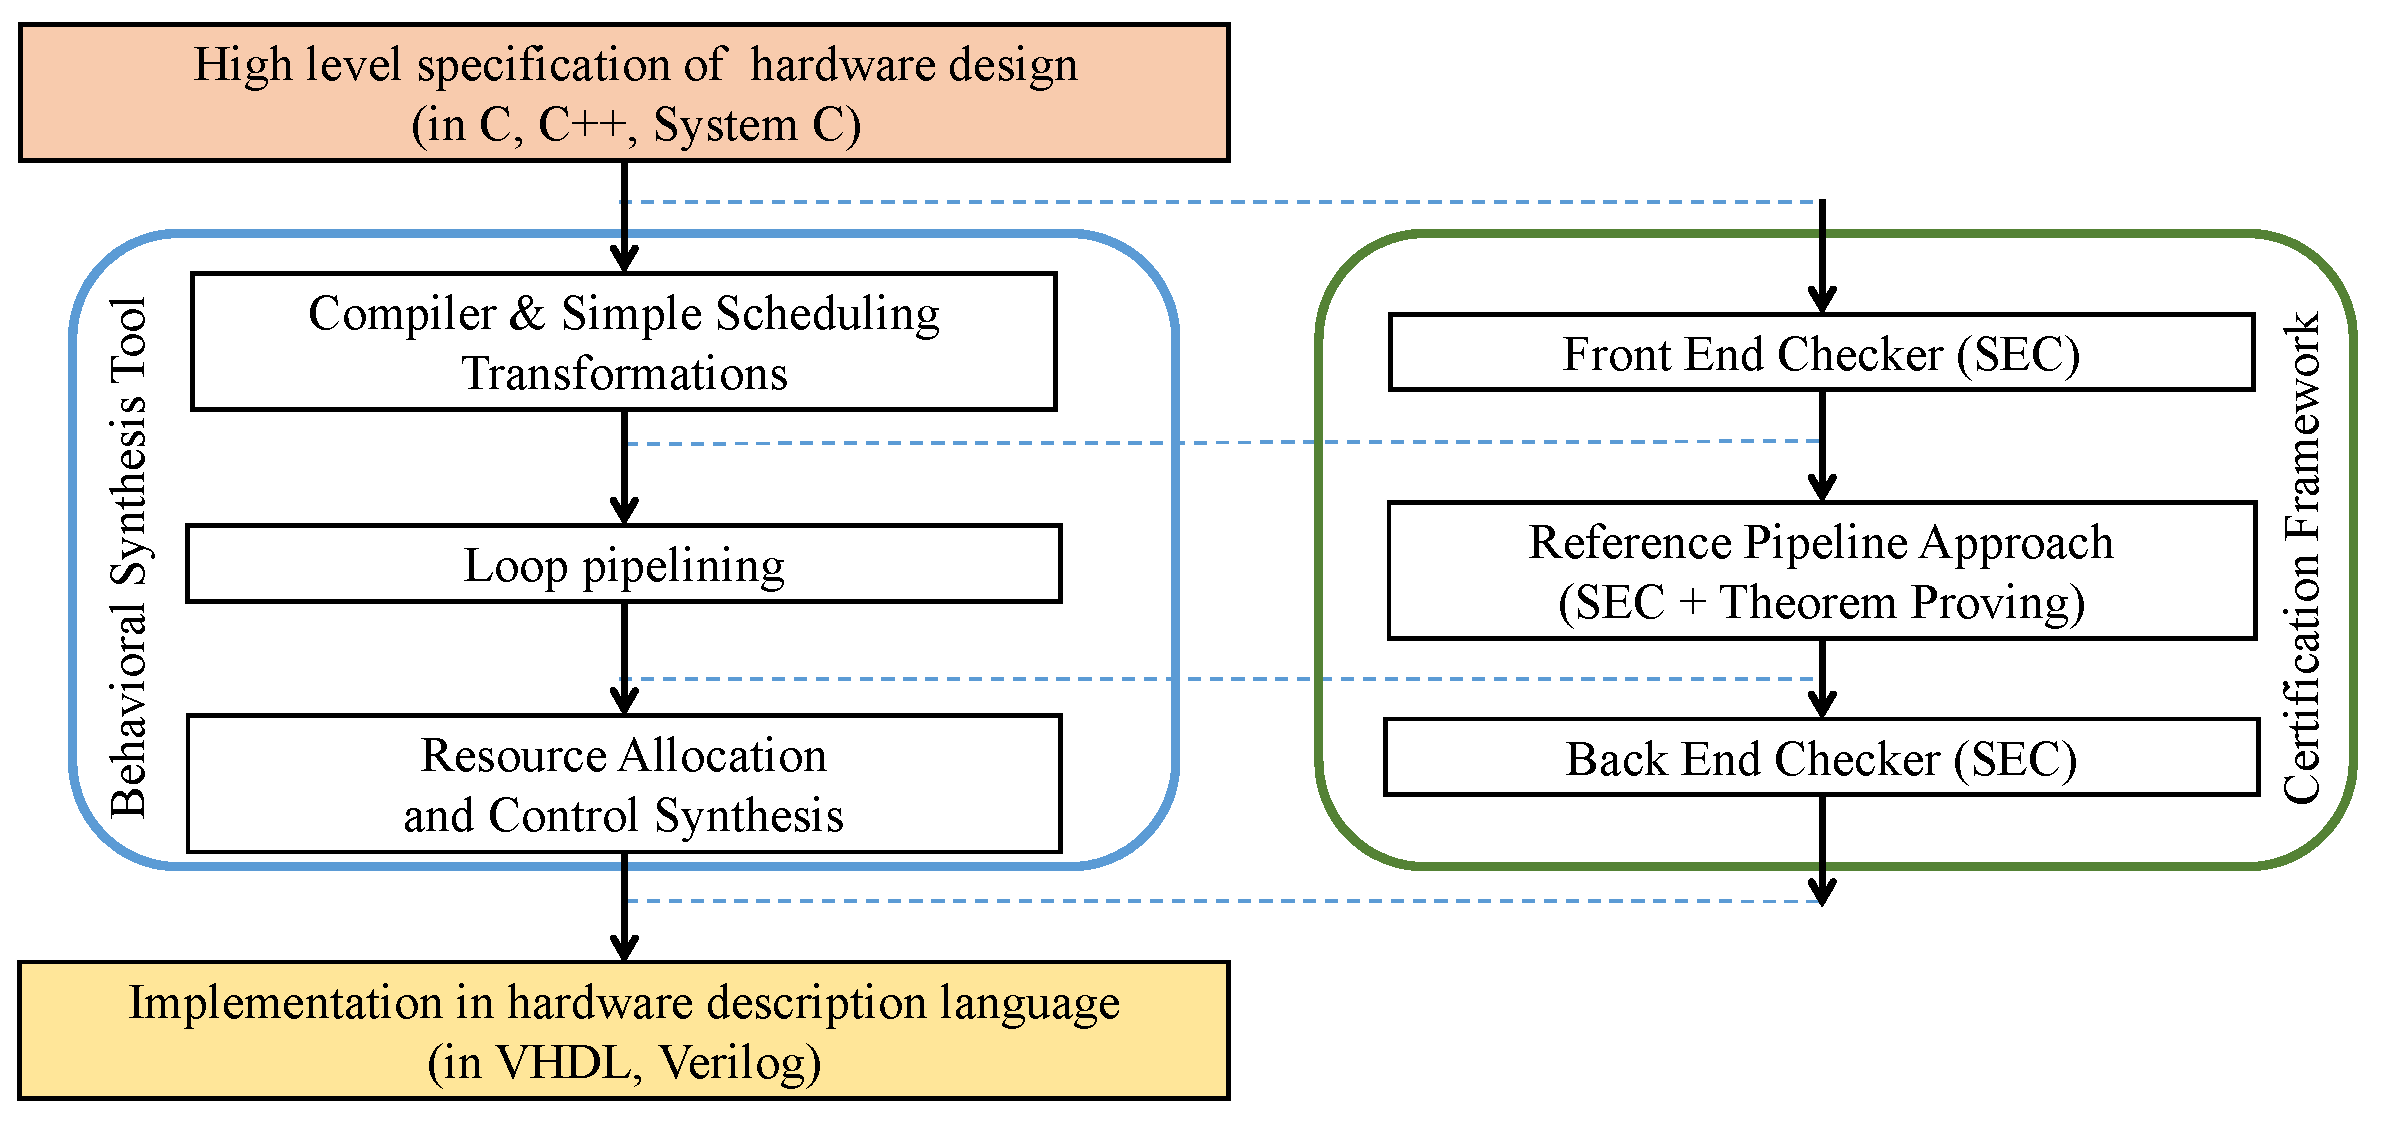
\includegraphics[height=2in]{fig-proposal/certification-framework}
\end{tabular}
\end{center}
\caption{Certification Model for Behaviorally Synthesized Pipelines}
\label{fig:certification-framework}
\end{figure}

The overall goal of the project is to provide a mechanized framework
for certifying hardware designs synthesized from ESL specifications by
commercial behavioral synthesis tools.
One obvious approach is to apply standard verification techniques (%\eg, 
SEC or
theorem proving) on the synthesized RTL itself.
Unfortunately, such a methodology is not practical.
As mentioned earlier, the large gap in abstraction
between the ESL and RTL descriptions means that there is little
correspondence in internal variables between the two.  Consequently,
direct SEC between the two reduces to cost-prohibitive computation of
input-output equivalence. On the other side, applying theorem proving
is also troublesome since extensive manual effort is necessary and
this effort needs to be replicated for each different synthesized
design. It is also infeasible to
directly certify the implementation of the {\em synthesis tool} via
theorem proving.  In addition to being highly complex and thus
potentially requiring prohibitive effort to formally verify with any
theorem prover, the implementations are typically closed-source and
closely guarded by EDA vendors and thus out of reach of external
automated reasoning communities.

To address this problem, previous work developed two key SEC
solutions, which we will refer to below as {\em Back-end} and {\em
Front-end}.  We then discuss the gap between them, which is being
filled by theorem proving efforts in this dissertation. The certfication model 
is illustrated in Figure~\ref{fig:certification-framework}.
\medskip

\noindent {\bf Back-end SEC:} The key insight behind
back-end SEC is that automated SEC techniques, while
ineffective for directly comparing synthesized RTL with the
top-level ESL description, are actually suitable to compare
the RTL with the intermediate representation (IR) generated
by the tools after the high-level (compiler and scheduling)
transformations have been applied.  In particular,
operation-to-resource mappings generated by the synthesis
tool provide the requisite correspondence between internal
variables of the IR and RTL.  Furthermore, a key insight is
that while the implementations of transformations are
unavailable for commercial EDA tools, most tools provide
these IRs after each transformation application together
with some other auxiliary information.  To exploit these, an
SEC algorithm was developed between the IR (extracted from
synthesis tool flow after these transformations) and
RTL~\cite{rhcxy:atva-09,hxry:date-10,kechengthesis,Yang2013}. 
The approach scales
to tens of thousands of lines of synthesized RTL.

\medskip

\noindent {\bf Front-end SEC:} Of course the back-end SEC
above is only meaningful if we can certify that the input
ESL indeed corresponds to the extracted IR produced after
the compiler and scheduling transformations applied in the
first two phases of synthesis. To address this, another SEC
technique was developed to compare two IRs~\cite{zhenkun:iccd-13,zhenkun2,zhenkun3}.  The idea then
is to obtain the sequence of intermediate representations
$\mbox{IR}_0,\ldots,\mbox{IR}_n$ generated by the compiler
and scheduling transformations, and compare each pair of
consecutive IRs with this new algorithm.  Then back-end SEC
can be used to compare $\mbox{IR}_n$ with the synthesized
RTL, completing the flow.

\bigskip

\noindent {\bf A Methodology Gap:} Unfortunately, the front-end SEC
algorithm can only compare two IRs that are structurally close.  If a
transformation significantly transforms the structure of an IR then
the heuristics for detecting corresponding variables between the two
IRs will not succeed, causing equivalence checking to fail.
Unfortunately, loop pipelining falls in the category of
transformations that significantly changes the structure of the IR.
It is a quintessential transformation that changes the control/data
flow and introduces additional control structures (%\eg, 
to eliminate
hazards).  This makes front-end SEC infeasible for its certification.
Furthermore, most commercial implementations are of course
proprietary and consequently not available to us for review; applying
theorem proving on those implementations is not viable from a
methodology perspective.  Thus a specialized approach is warranted for
handling its certification.



\section{Formalization}
\label{sec:formalization}

\subsection{Intermediate Representation}
\label{subsec:ir}

A behavioral synthesis tool performs a number of compiler
and scheduling transformations (including pipelining). Certification of behavioral synthesis transformations thus requires a formalization of
the design representation manipulated by these
transformations. The formalization we use is {\em Clocked
  Control Data Flow Graph} (CCDFG)~\cite{rhcxy:atva-09}. 
Structurally, a CCDFG is a control and data flow graph augmented with a schedule. The control flow is broken into basic blocks. The instructions are grouped into microsteps which can be executed concurrently. A scheduling step represents a group of microsteps which can be executed in a single clock cycle. State of a CCDFG at a particular microstep is a list of all the variables of a CCDFG with their corresponding values.  The semantics of CCDFG require a formalization of the
underlying language used to represent the individual
instructions in a scheduling step.  The underlying language we use
is the LLVM language~\cite{llvm}. LLVM is a popular compiler
infrastructure for many behavioral synthesis tools~\cite{autoesl,xpilot} and includes an assembly language front-end.  We currently support
only a subset of LLVM operations which are required to handle all the designs we have
seen.  Instructions supported include assignment, load,
store, bounded arithmetic, bit vectors, arrays, and pointer
manipulation instructions.  Note that the reasoning involved 
in creating a pipelined CCDFG does not involve the exact 
syntax of any operation. We are merely concerned with a way 
to find the variables which are read and written at each step.
Increasing the operations database in our algorithm 
is expected to increase the time taken to prove certain primitives as much 
more analysis needs to be done.
However, it would not affect the logical reasoning of the primitives, the overall
algorithm and the proof.  
We define the syntax of each
type of statement by defining an ACL2 predicate.  For
example as shown in Figure~\ref{fig:syntax}, in our syntax, an {\em assignment statement} can be
expressed as a list of a variable and an
expression. An expression can further be of multiple types, %\eg, 
{\em load expression} (loading the value of a variable from memory), {\em add
expression} (addition of two variables), {\em xor expression} (xor of two variables)
etc., where each expression includes the operation applied to the
appropriate number of arguments. We provide semantics to these instructions through a
state-based operational formalization as is common with
ACL2~\cite{liu}. We define the notion of a CCDFG state, which includes
the states of the variables, memory, pointers, etc.  Then we
define the semantics of each instruction by specifying how
it changes the state.  Thus, for an assignment statement we
will have a function {\em execute-assignment} that specifies
the effect of executing the assignment statement on a CCDFG
state.

\begin{figure}
\begin{center}
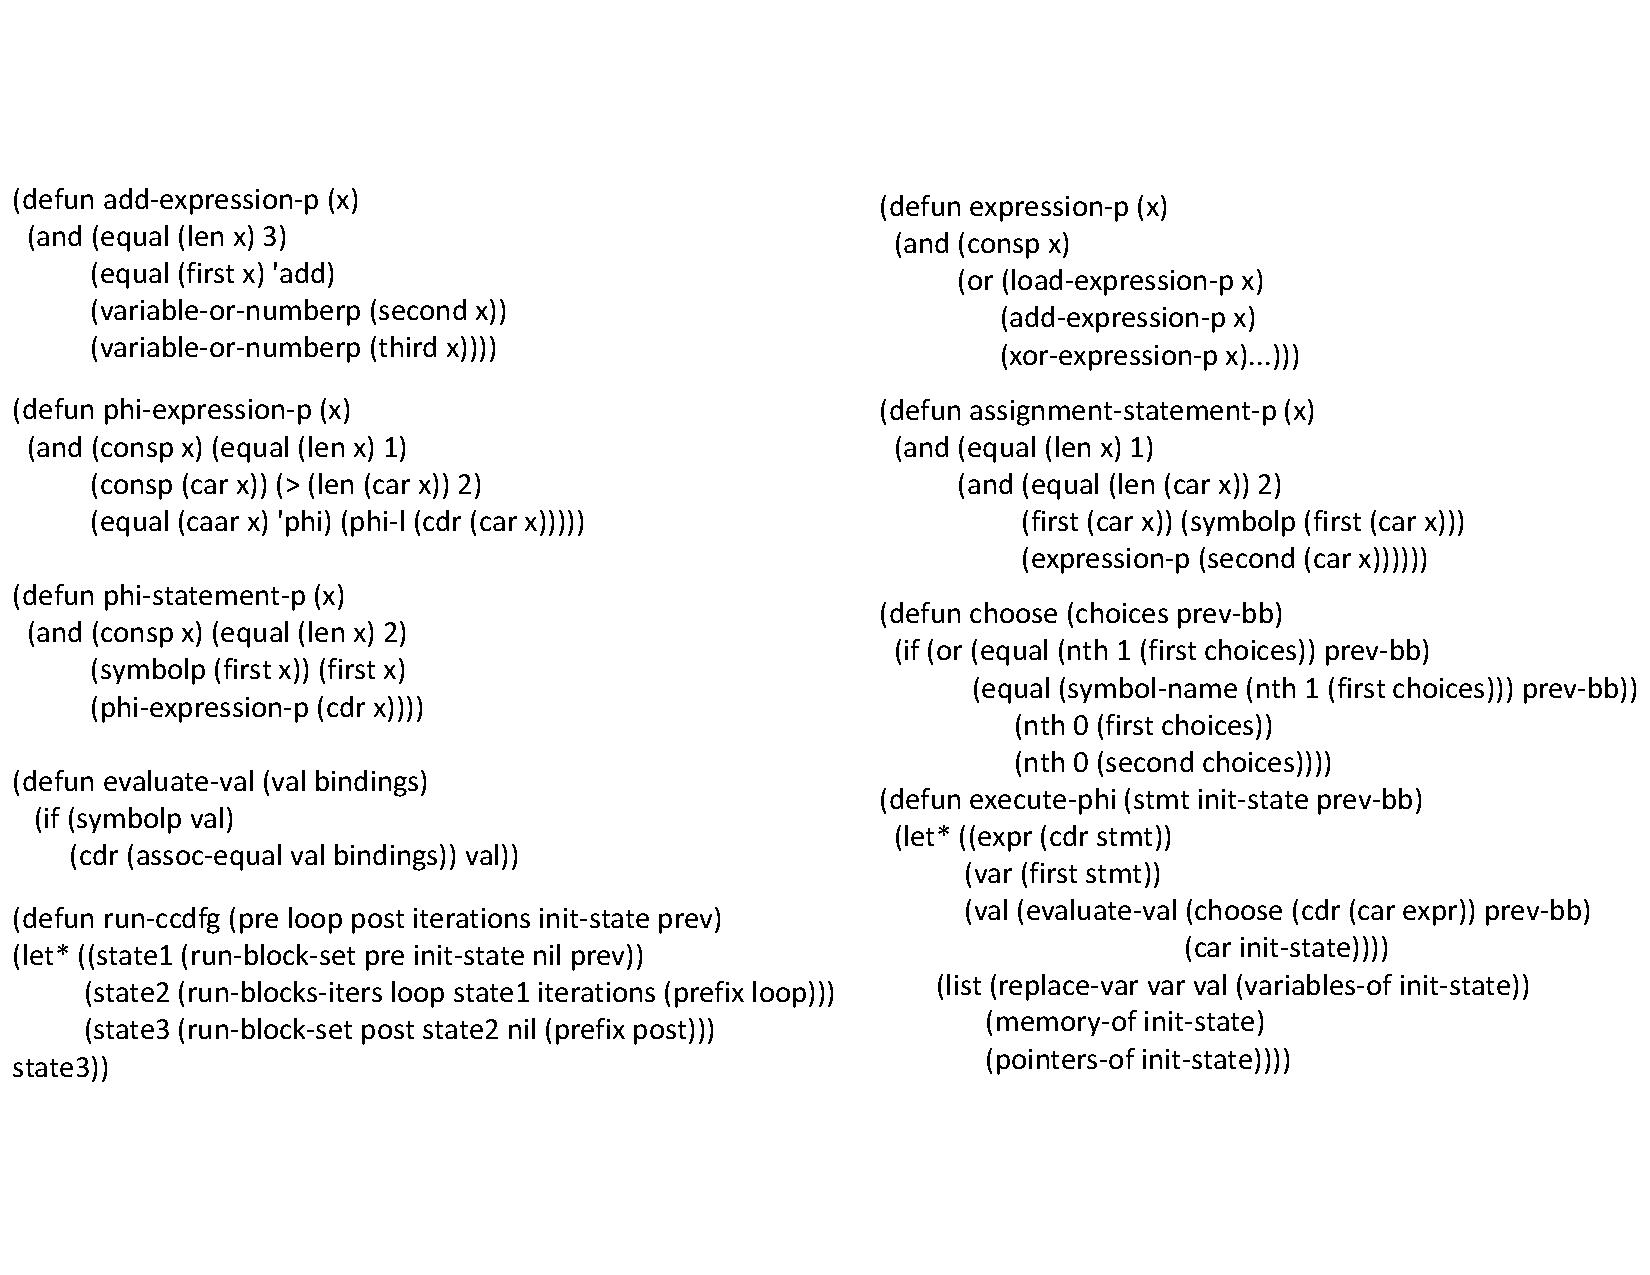
\includegraphics[width=4.5in]{fig-proposal/formalization1}
\end{center}
\caption{Modelling programming Language constructs in ACL2}
\label{fig:syntax}
\end{figure}

Defining the semantics of most supported statements is straightforward, with one exception.  The exception is the so-called ``$\phi$-construct'' available in LLVM~\cite{llvmphi}.  A $\phi$-construct is a list of $\phi$-statements.  A $\phi$-statement is $v := \phi [\sigma, bb1] [\tau, bb2]$, where $v$ is a variable, $\sigma$ and $\tau$ are expressions, and $bb1$ and $bb2$ are basic blocks: if it is reached from $bb1$ then it is the same as the assignment statement $v := \sigma$; if reached from $bb2$, it is the same as $v := \tau$; the meaning is undefined otherwise. The construct is complex since the effect of executing this statement on a CCDFG state $s$ depends not only on the state $s$ but also on how $s$ is reached by the control flow. Unfortunately, $\phi$-statements are required in loop designs --- they are used to evaluate the value of loop carried dependencies. Consequently, the complexity induced by this instruction cannot be avoided. 

%\small
%\begin{verbatim}
%(defun phi-expression-p (x)
 % (and (consp x) (equal (len x) 1)
%       (consp (car x)) (> (len (car x)) 2)
 %      (equal (caar x) 'phi) (phi-l (cdr (car x)))))

%(defun phi-statement-p (x)
%  (and (consp x) (equal (len x) 2)
%       (symbolp (first x)) (first x)
%       (phi-expression-p (cdr x))))
%\end{verbatim}
%\normalsize

In Figure~\ref{fig:syntax}, in function {\em phi-expression-p}, {\tt phi-1} recognizes an expression of the form {\tt
  ((E0 b) (E1 b-prime))} where {\tt E0} and {\tt E1} are
expressions and {\tt b} and {\tt b-prime} are symbols
representing basic blocks.  Thus in ACL2, the
$\phi$-statement looks like {\tt (v (phi ((E0 b) (E1
  b-prime))))}.  Finally, the execution semantics requires
the additional parameter {\tt prev-bb} to track the previous
basic block. In {\em execute-phi}, the {\em init-state} represents the state of a CCDFG before executing $\phi$-statement. The function 
{\em variables-of} is used to get a list of all the variables of {\em init-state} with their corresponding values. 
{\em replace-var} replaces the values of the variable {var} to {val} in the list of those variables.
%Function definition for execute-phi uses the functions
%%evaluate-val, replace-val and variables-of which are not
%%explained.

%\small
%\begin{verbatim}
%(defun choose (choices prev-bb)
% (if (or (equal (nth 1 (first choices)) prev-bb)
%          (equal (symbol-name (nth 1 (first choices))) prev-bb))
%      (nth 0 (first choices))
%    (nth 0 (second choices))))
    
%(defun evaluate-val (val bindings)
 % (if (symbolp val) 
 %     (cdr (assoc-equal val bindings)) 
 %   val))

%(defun execute-phi (stmt init-state prev-bb)
%  (let* ((expr (cdr stmt))
 %        (var (first stmt))
 %        (val (evaluate-val (choose (cdr (car expr)) prev-bb) 
 %                                  (car init-state))))
 %   (list (replace-var var val (variables-of init-state)) 
 %         (memory-of init-state) 
 %         (pointers-of init-state))))         
%\end{verbatim}
%\normalsize

%% Added
%The {\em init-state} represents the state of a CCDFG before executing $\phi$-statement. The function 
%{\em variables-of} is used to get a list of all the variables of {\em init-state} with their corresponding values. 
%{\em replace-var} replaces the values of the variable {var} to {val} in the list of those variables.

%.
%({\em e.g.}, AutoESL~\cite{autoesl}, xPilot~\cite{xpilot}).  
%We provide semantics to these instructions through a standard, state-based operational formalization~\cite{McCarthy}. It includes assignment, load, store, bounded arithmetic, bit ve XXX shows the formalization of a few instructions in ACL2.  As is standard with ACL2, the formalization specifies the effect  of execution of each instruction on the underlying abstract machine state based on the CCDFG representation.Executing a microstep ina CCDFG implies changing the current state of CCDFG based onmeaning of the instructions in the microstep and producing anew state. %Assigning meanings to most instructions is
%standard; one exception is the so-called ``$\phi$-construct''. A $\phi$-construct is a list of $\phi$-statements. A $\phi$-statement is $v := \phi [\sigma, X] [\tau, Y]$, where $v$ is a variable, $\sigma$
%and $\tau$ are expressions, and $X$ and $Y$ are
%scheduling steps: if it is reached from $X$ then it is the
%same as the assignment statement $v := \sigma$; if
%reached from $Y$, it is the same as $v := \tau$; the meaning is undefined otherwise. $\phi$-constructs are necessary due to the structure of the SSA (static single
%assignment) form of the LLVM code.

\subsection{Correctness of Loop Pipelining}
%A behavioral synthesis tool automatically generates a RTL design from an ESL design through a series of
%transformations. Pipelining a loop is a critical
%transformation in behavioral synthesis.
%\begin{enumerate}
%\item no nested loop;
%\item only one $Entry$ and one $Exit$ block; and
%\item no branching between the scheduling steps.
%\end{enumerate}

For the purposes of this paper, a {\em pipelinable loop} is a loop with the following restrictions~\cite{hrx:dac-12}: (1) no nested loop; 
(2) only one $Entry$ and one $Exit$ block; and (3) no branching between the scheduling steps.  
Our well-formed pipelinable loop has only one conditional branch and one unconditional branch. 
Unconditional branch is at the end of the loop dictating the back edge which enforces that the loop CCDFG is executed again from the first step. 
Conditional branch ensures that depending on the current value of the exit condition variable, a loop can exit if required. 
Other intermediate branches have already been handled by compiler and scheduling transformations prior to the pipelining transformation
so we need not consider them in our reasoning. There is one {\em $\phi$-construct}~\cite{llvmphi} in the first scheduling step which handles the value assigned
to loop carried variables depending on whether we are entering loop for the first time or not. These restrictions are not just meant to simplify the problem, but reflect the kind of loops that can be actually pipelined during behavioral
synthesis. For instance, synthesis tools typically require inner loops to have been fully unrolled (perhaps by a previous compiler
transformation) in order to pipeline the outer loop.

\begin{figure}[H]%[t!]
\begin{center}
\begin{tabular}{cc}
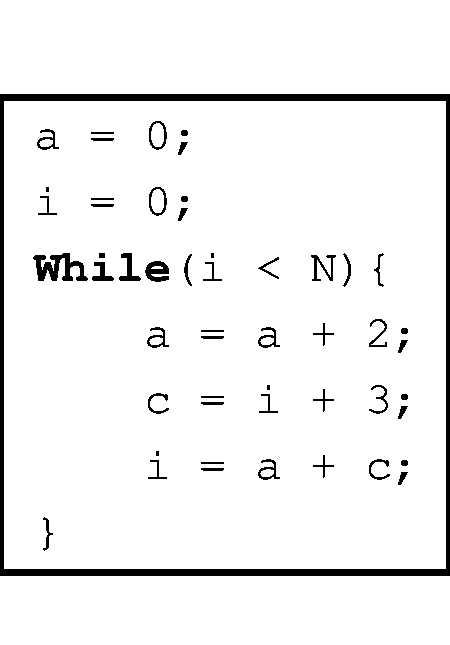
\includegraphics[height=1.5in]{fig-rpe/C-code}
& \hspace{2cm}
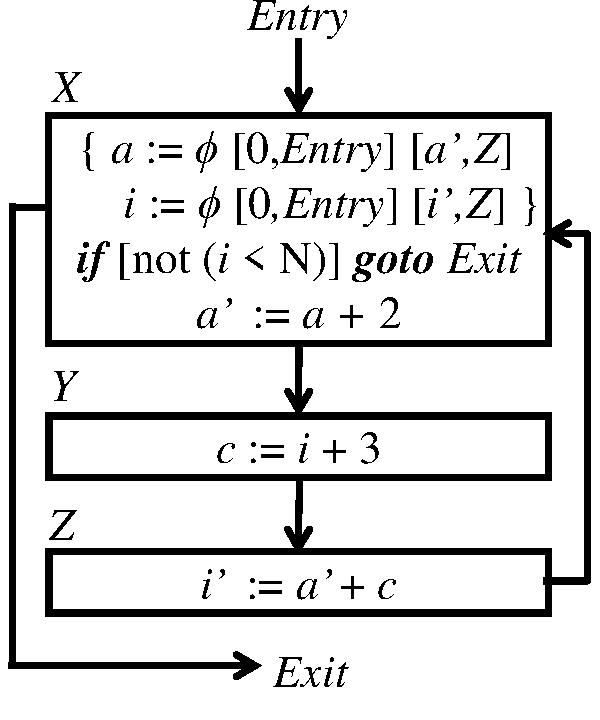
\includegraphics[height=1.5in]{fig-rpe/seq-ccdfg}
\\
(a) & \hspace{2cm} (b) 
\end{tabular}
\end{center}
\caption{(a) Loop in C (b) Loop CCDFG before pipelining.}
\label{fig:high-level-synthesis-1}
\end{figure}

Figure~\ref{fig:high-level-synthesis-1}(a) illustrates the C
code (ESL description) for a loop.  The C code does not have
a schedule or the concept of a clock cycle.
Figure~\ref{fig:high-level-synthesis-1}(b) shows CCDFG of the
sequential loop just before loop pipelining. The loop has
three scheduling steps: $X$, $Y$ and $Z$.  The scheduling
step before the loop is $Entry$ and after the loop is
$Exit$. The edges  in the CCDFG indicate the control flow.
Note that the sequential CCDFG has Static Single Assignment (SSA) structure
, as a result variable $a$ and $i$ are not assigned 
more than once and we require the quoted variables $a'$ and $i'$.

%% Since, reasoning about execution becomes difficult if we have to
%% always keep track of the previous scheduling step, we treat the first
%% iteration of the sequential CCDFG {\em seq-pre-loop} as a separate
%% iteration than the rest of the iterations {\em seq-loop}.  Infact, the
%% first step of our pipelining algorithm is to unroll the loop once and
%% replace $\phi$-construct by corresponding assignment statements based
%% on the previous scheduling steps.

%% \subsection{Correctness Statement}
%% \label{subsec:correctness-defn}

%% IMPORTANT : take a look again, if we want to keep all iterations same, we can start from k = 0

The main lemma involved in the correspondence proof between
the sequential and pipelined CCDFG can be paraphrased in English as follows. 

\begin{quote}
 If the pipeline generation succeeds without error,
 executing the pipelined CCDFG loop for $k$ iterations
 generates the same state of the relevant variables as
 executing the sequential CCDFG for some $k'$ iterations.
 The explicit value of $k'$ is given by the term {\tt (+ (-
   k 1) (ceil m pp-interval))}.
 \end{quote}

The theorem can be stated in ACL2 as follows.
%\footnote{The theorem mentioned in the paper does not contain all the hypotheses. Please refer to our proof scripts for final form of this theorem.}

\small
\begin{verbatim}
    
(defthm correctness-statement-key-lemma
    (implies (and (posp k)
                  (posp pp-interval)
                  (posp m)
                  (equal pp-ccdfg 
                     (superstep-construction pre loop pp-interval m))
                  (not (equal pp-ccdfg "error"))))
    (equal (in-order (get-real (run-ccdfg (first pp-ccdfg) 
                                         (second pp-ccdfg) 
                            	            (third pp-ccdfg) 
                            	            k init-state prev)))
              (in-order (run-ccdfg pre loop nil 
								               		                  (+ (- k 1) (ceil m pp-interval)) 
                                 		init-state prev)))))
\end{verbatim}
\normalsize

The theorem involves several ACL2 functions, \eg,
{\tt get-real}, \\ {\tt superstep-construction}, etc. 
%We do not
%discuss the detailed definitions of these functions in the
%paper, but they are available with the supporting ACL2
%script for this workshop.  
We provide a brief, informal
description of some of the critical functions in the theorem.
Two key functions that appear in the theorem above are {\tt
  superstep-construction} and {\tt run-ccdfg}. The function {\tt run-ccdfg} (refer Figure~\ref{fig:syntax}) runs a CCDFG including a
pipelinable loop in three parts, first the prologue before the
loop, next the loop itself, and finally the epilogue past the
loop.
%\footnote{Of course one can have the standard function {\tt run} that executes the entire CCDFG rather than in parts.  However, for reasons that will be clear when we define the invariant, in our case it is easier to do most of the work with the execution in three parts and then assemble them into a final theorem about the CCDFG run in the end.}  
The function {\tt superstep-construction} combines the scheduling steps of successive iterations to create the ``scheduling supersteps'' of pipelined CCDFG.  If there are data-hazards and pipelined CCDFG cannot be generated as per
the pp-interval given, the function generates an ``error''.
Finally, the function {\tt get-real} removes from the
pipelined CCDFG state, all auxiliary variables introduced by
the pipeline generation algorithm itself, leaving only the
variables that correspond to the sequential
CCDFG,
%\footnote{The algorithm has to introduce new variables in order to eliminate hazards.  One consequence of this is that the new variables so introduced must not conflict with any variable subsequently used in the CCDFG.  Since we do not have a way to ensure generation of fresh variables, this constraint has to be imposed in the hypothesis.}  
and {\tt in-order} normalizes ``sorts'' the
components in a CCDFG state in a normal form so that the
sequential and pipelined CCDFG states can be compared with
{\tt equal}.
  %This function is defined as follows, where {\tt
  %prefix} determines the previous scheduling step of the
%iteration (required to resolve $\phi$-statements).

%\begin{verbatim}
%(defun run-ccdfg (pre loop post iterations init-state prev)
%  (let* ((state1 (run-block-set pre init-state nil prev))
 %        (state2 (run-blocks-iters loop state1 iterations (prefix loop)))
 %        (state3 (run-block-set post state2 nil (prefix post)))
 %   state3))
%\end{verbatim}




%\smallskip
%\noindent {\textbf {Correctness Statement:}}
%Let $L$ be a loop in CCDFG $C$, and let $L_{\alpha}$ be the
%pipelined implementation generated by a pipeline algorithm using
%pipeline parameters $\alpha$.  Let $V$ be the set of
%variables in $L$, and $U$ be the set of all
%variables in $C$.  Suppose we execute $L$ and $L_{\alpha}$
%from CCDFG states $s$ and $s'$ respectively, such that for
%each variable $v\in V$, the value of $v$ in $s$ is the same
%as that in $s'$, and suppose that the state on termination
%are $f$ and $f'$ respectively.  Then (1)~for any $v\in V$,
%the value of $v$ in $f$ is the same as that in $f'$, and
%(2)~for any $v\in(U\backslash V)$, the value of $v$ in $f'$
%is the same as that in $s'$.

%\medskip
%\noindent
%{\em Remark:} Condition (2)
%ensures that variables in $C$ that are not part of the loop
%are not affected by $L_{\alpha}$.  The value of any new
%variables introduced by the algorithm in $f'$ are irrelevant since they are not accessed
%subsequently.



%\subsection{Loop Pipelining Transformation}
%\label{subsec:loop-pipelining-trans}
%For our purposes, {\em pipelinable loop} is a loop with the following additional restrictions~\cite{hrx:dac-12}:
%\begin{enumerate}
%\item no nested loop;
%\item only one $Entry$ and one $Exit$ block; and
%\item no branching between the scheduling steps.
%\end{enumerate}
%These restrictions reflect the kind of loops that can be actually pipelined during behavioral synthesis. For instance, synthesis tools typically require inner loops to have been fully unrolled  in order to pipeline the outer loop.


%\begin{figure}[H]%[t!]
%\begin{center}
%\begin{tabular}{cc}
%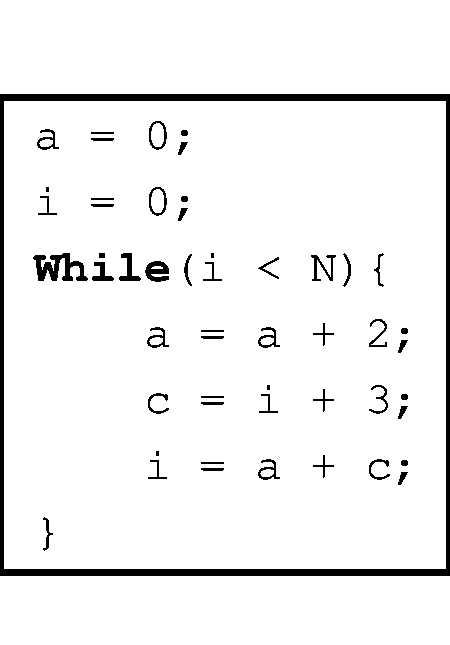
\includegraphics[height=1.5in]{fig-rpe/C-code}
%& \hspace{2cm}
%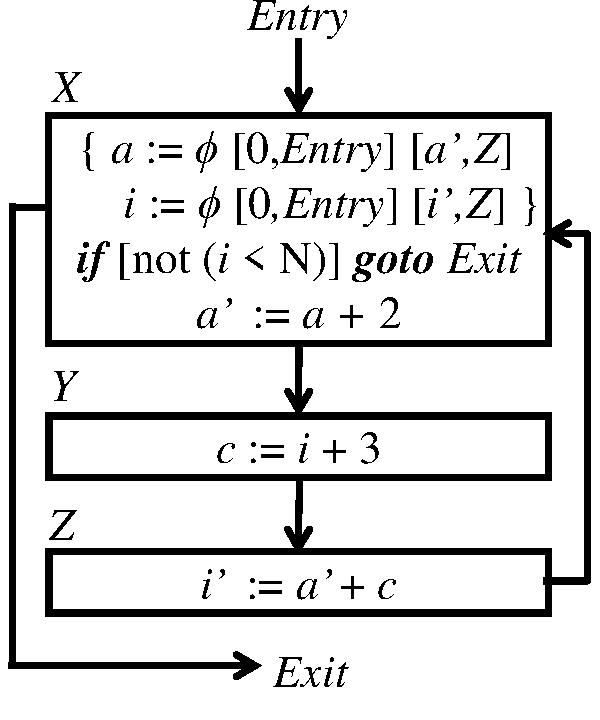
\includegraphics[height=1.5in]{fig-rpe/seq-ccdfg}
%\\
%(a) & \hspace{2cm} (b) 
%\end{tabular}
%\end{center}
%\caption{(a) Loop in C (b) Loop CCDFG before pipelining.}
%\label{fig:high-level-synthesis}
%\end{figure}

%Figure~\ref{fig:high-level-synthesis}(a) illustrates the C code for a loop at the beginning of the synthesis process. The C code does not have a schedule or the concept of a clock cycle. Figure~\ref{fig:high-level-synthesis}(b) shows CCDFG of the sequential loop just before loop pipelining. The loop has three scheduling steps: $X$, $Y$ and $Z$.  The scheduling step before the loop is $Entry$ and after the loop is $Exit$. Since, there are three scheduling steps in the loop, one iteration can be executed in three clock cycles.

%\begin{figure}
%\begin{center}
%\begin{tabular}{cc}
%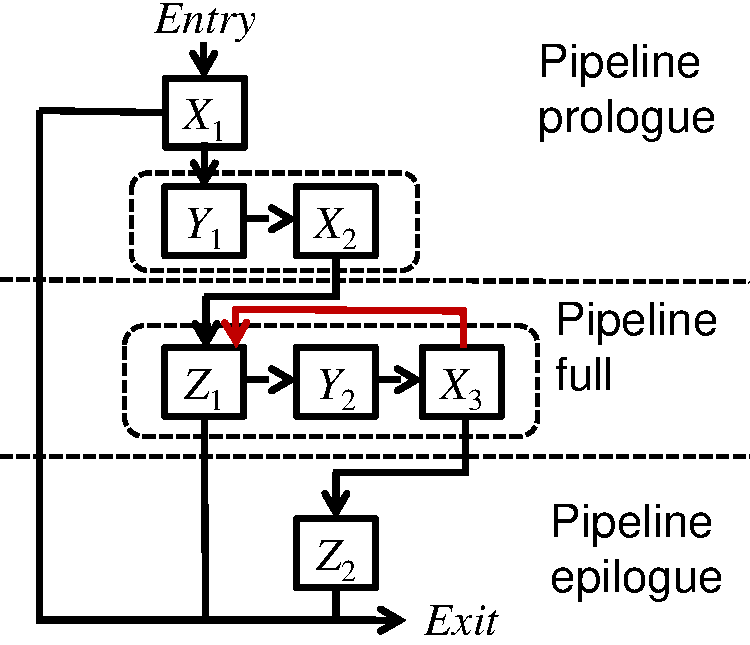
\includegraphics[height=1.5in]{fig-rpe/pipelined_ccdfg}
%& \hspace{0.5cm}
%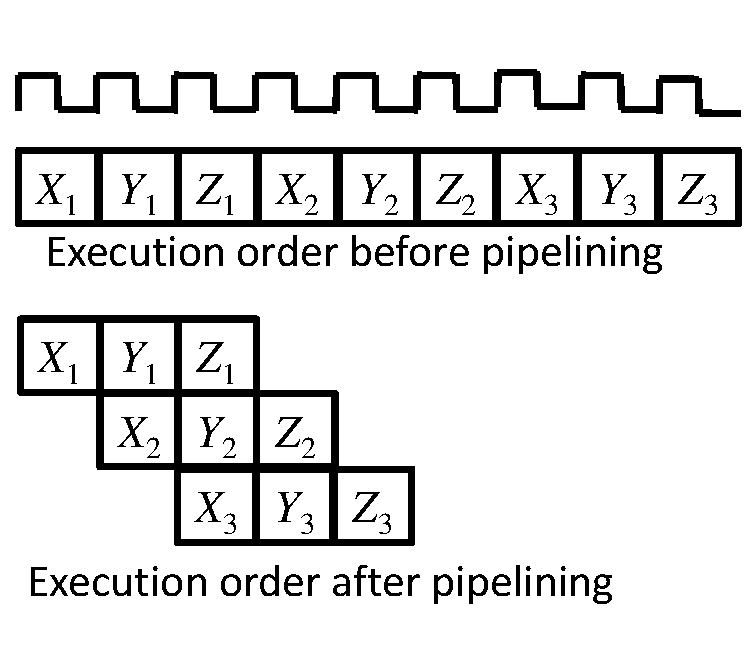
\includegraphics[height=1.5in]{fig-rpe/pp-clock-cycles}
%\end{tabular}
%\end{center}
%\caption{Pipelined CCDFG. The horizontal arrows indicate data forwarding.}
%\label{fig:pp-ccdfg}
%\end{figure}

%:Behavioral synthesis tools use complicated heuristics and aggressive scheduling strategies to find an optimized pipeline interval (clock cycles after which a new iteration can be started such that there are no data hazards). Figure~\ref{fig:pp-ccdfg} shows the pipelined CCDFG with a pipeline interval equal to one. The new scheduling steps in the pipelined CCDFG created by combining scheduling steps from different iterations of the sequential CCDFG are called scheduling supersteps. Observe that the three iterations of the pipelined loop take five clock cycles as opposed to nine clock cycles in the sequential loop. Loop pipelining reduces the number of clock cycles required to execute the loop, hence this transformation is used by synthesis tools to increase throughput and reduce latency.  

%\subsection{Correctness of Pipelined CCDFG}
%\label{subsec:correctness-defn}

%Correctness of loop pipelining can be informally stated as below.

%\begin{quote}
%Let $L$ be a loop in CCDFG $C$, and let $L_{\alpha}$ be the pipelined loop CCDFG. Let $V$ be the set of variables mentioned in $L$, and $U$ be the set of all variables in $C$.  Suppose we execute $L$ and $L_{\alpha}$ from CCDFG states $s$ and $s'$ respectively, such that for each variable $v\in V$, the value of $v$ in $s$ is the same as that in $s'$, and suppose that the state on termination are $f$ and $f'$ respectively.  Then (1)~for any $v\in V$, the value of $v$ in $f$ is the same as that in $f'$, and (2)~for any $v\in(U\backslash V)$, the value of $v$ in $f'$ is the same as that in $s'$.
%\end{quote}
%\noindent
%{\em Remark:} Condition (2) is the {\em frame rule} which ensures that variables in $C$ that are not part of the loop are not affected by $L_{\alpha}$.


\section{Research Challenges}
\label{sec:challenges}

To understand the complexities involved in mechanical
certification of an algorithm that was not designed
originally with certification in mind, we need to re-visit
the general approach to applying formal reasoning on
software programs.  The typical approach is to break the
program into a number of pieces, prove key lemmas
characterizing the role of each piece, and then chain these
lemmas together into a proof of the correctness of the
entire program. Crucial to this approach, however, is the
requirement that each program piece can be characterized by
a succinct invariant that can be easily verified.  However,
in a program not developed with reasoning in mind,
optimizations typically destroy the structural disciplines
and modularity of the individual program pieces. This makes it
difficult to identify and isolate the components that
actually maintain succinct, interesting invariants.


Our first approach was to certify their implementation as it is using theorem proving. But, our experience was that it is a difficult approach, one that we need not endure. In general, in order to certify such an arbitrary implementation,
one has to either (1)~restructure the implementation into
one that is more disciplined, and prove the equivalence
between the two, or (2)~come up with very complex
invariants that essentially comprehend how invariants from
each individual piece are conflated together in the
implementation.  Both approaches require extensive human
interaction, resulting in the proverbial euphemism of proofs
of programs being orders of magnitude more complex than the
programs themselves~\cite{liu}.

In our work, however, we can ``get away'' without verifying
the specific implementation while still being able to
certify the design generated by behavioral synthesis without
loss of fidelity. The key observation, as above, is that it
is sufficient to develop {\em any} certifiable algorithm
that generates a pipelined CCDFG from a sequential
implementation which can be effectively applied with SEC.
In particular, any certifiable algorithm that has the same
input-output characteristic as the proposed algorithm
is sufficient.  Thus, our work is on identifying
certifiable primitives and invariants of a loop pipelining
transformation and developing a pipeline generation
algorithm using those primitives, achieving the dual goal of
mechanical reasoning of the algorithm and amenability of the
resulting reference model to SEC.

Note that our framework is independent of the inner workings of a specific tool, and can be applied to certify designs synthesized by different tools from a broad class of ESL descriptions. Also, the approach produces a certified reference flow, which makes explicit generic invariants that must be preserved by different transformations. Checking correctness using formal methods prompted us to address the issues lacking in the previous algorithm. To ensure that control flow is maintained, we had to deal with branches. The previous algorithm introduces the concept of Exit edges but does not explain/implement them. The previous authors checked the output of their algorithm with RTL under the assumption that the loop never exits, hence they did not face any issue while testing. However, removing a conditional branch in a loop and furthermore, adding the conditional branch back in the middle of a pipelined loop requires complex reasoning which we manage using one of our primitives, explained in Chapter~\ref{sec:pipelining-algorithm}.

Also, the invariant that data flow is maintained at each step enabled us to find a bug in the previous algorithm. The previous algorithm moves a statement to make sure one particular data hazard is removed, but in doing so they move the statement across a conditional branch statement. Our primitves ensure that such a move is not possible. We have restructred the algorithm so that instead of going across a conditional branch in the same iteration, the movement of step is now to the previous iteration, explained in Chapter ~\ref{sec:pipelining-algorithm}. 



\section{Our Approach}
\label{sec:pipelining-algorithm}

Pipeline synthesis is based on the key observation that
successive iterations can be overlapped without affecting execution as long
as data and control dependecies are correctly maintained. 
Thus, the three main
activities of a pipeline synthesis algorithm are to
(1)~identify and remove possible hazards (2)~overlap the
successive iterations according to the pipeline interval, and 
(3)~ensure proper placement of conditional and unconditional branches. In our case,
the identification of data hazards is simplified since the synthesis tool
provides a pipeline interval. If we can use this pipeline interval to build our design, 
then the pipeline reference model is comparable to RTL in abstraction. 

We have developed a framework of five certified pipelining
primitives which allows us, among other things, to prevent possible data
hazards. Our framework also provides a primitive
to overlap successive iterations and a provision to add and remove 
branches when required while still maintaining the control flow. We now discuss
the framework in detail.

\subsection{Framework of Provable Pipelining Primitives}

We believe that the following primitives are necessary and essential in creating any pipelining
algorithm in behavioral synthesis.

{\textbf {$\phi$-elimination primitive}} -- 
Reasoning about the $\phi$-statement is complex since after its
execution from a state, say $s$, the state reached depends not only
on the state $s$ but also on previous basic blocks in the execution history.
However, we must handle it since it is used extensively in
loops to perform different actions depending on whether the
loop body is executed the first time. One of the key steps in loop pipelining is,
therefore, $\phi$-elimination {\em i.e.}, replacing
$\phi$-statement with appropriate assignment statements when the previous basic block is known.

{\textbf {Shadow register primitive}} -- We define a shadow register microstep as an assignment
statement with symbol expression ($x$) assigned to a new value ($x\_reg$). We call all the new introduced 
variables as shadow registers. Intuitively, it is correct that in a sequence of steps, if we assign a variable 
to a shadow register and replace all occurences of $x$ with $x\_reg$
till the next write of $x$, we should
not have made any difference in the execution. Also, since we are not changing the value of $x$ itself, 
the state after end of execution for both CCDFGs as far as real variables are concerned (all variables
 excluding all shadow registers) is same. 

\begin{figure}[H]
\begin{center}
\begin{tabular}{cc}
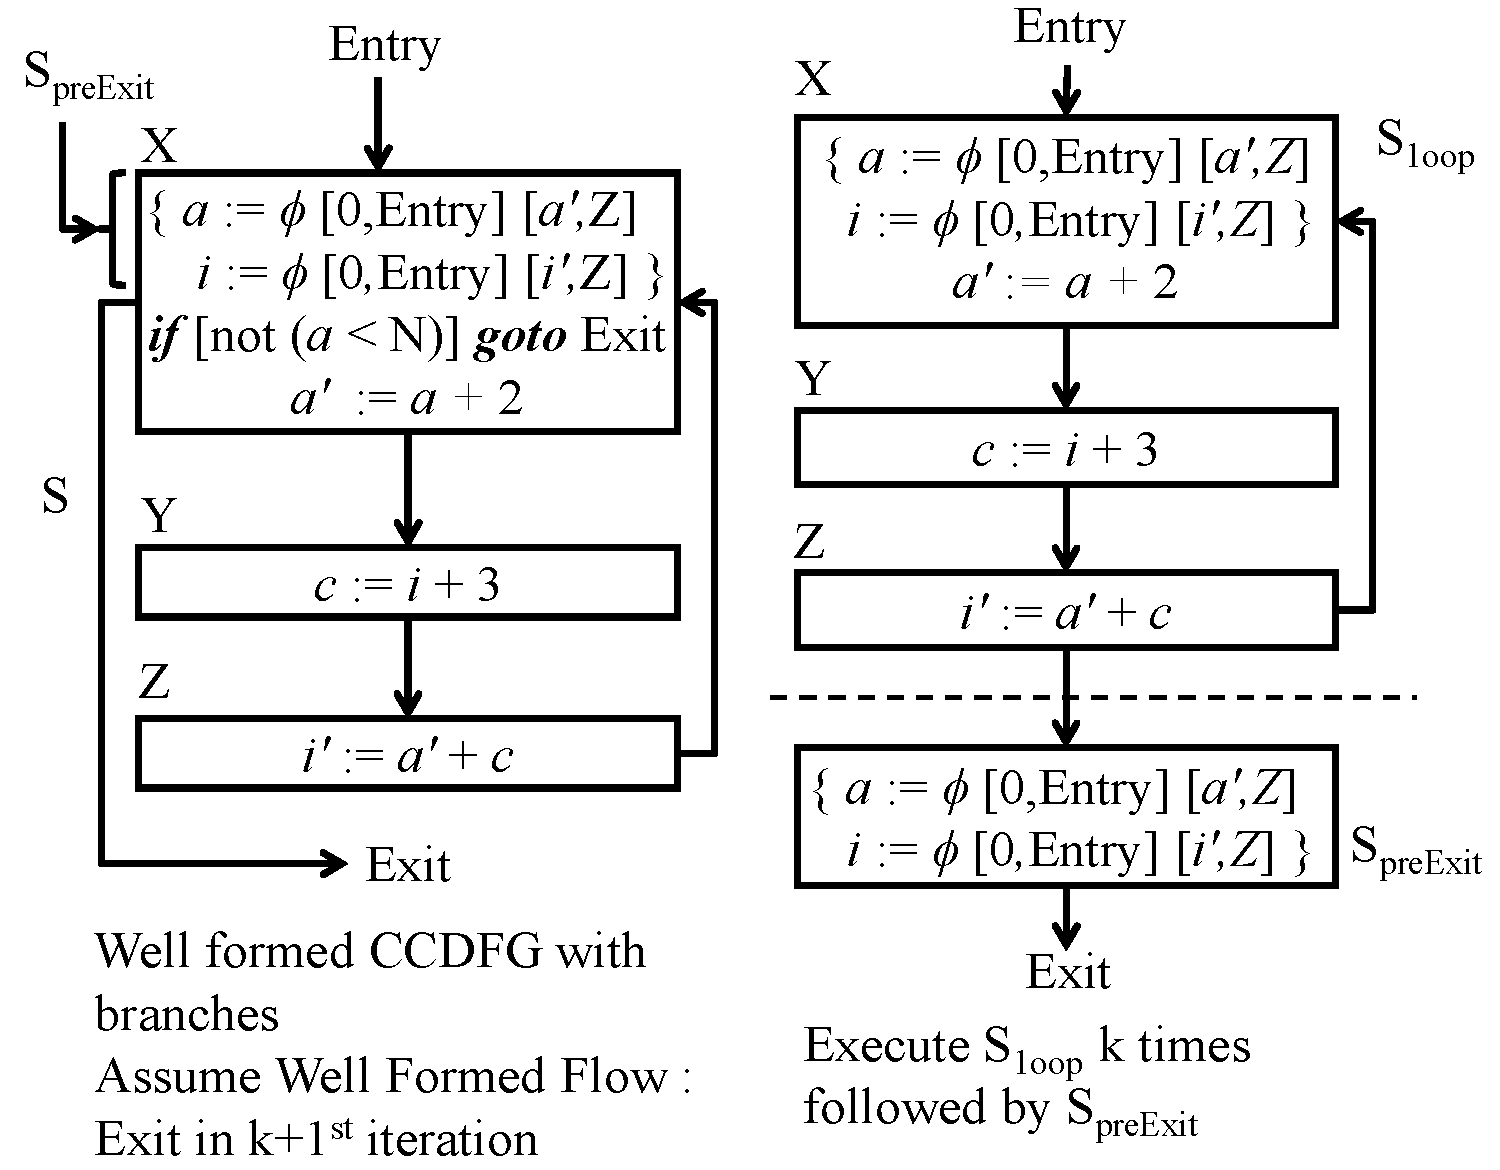
\includegraphics[height=1.8in]{fig-proposal/conditional-branch-primitive}
& 
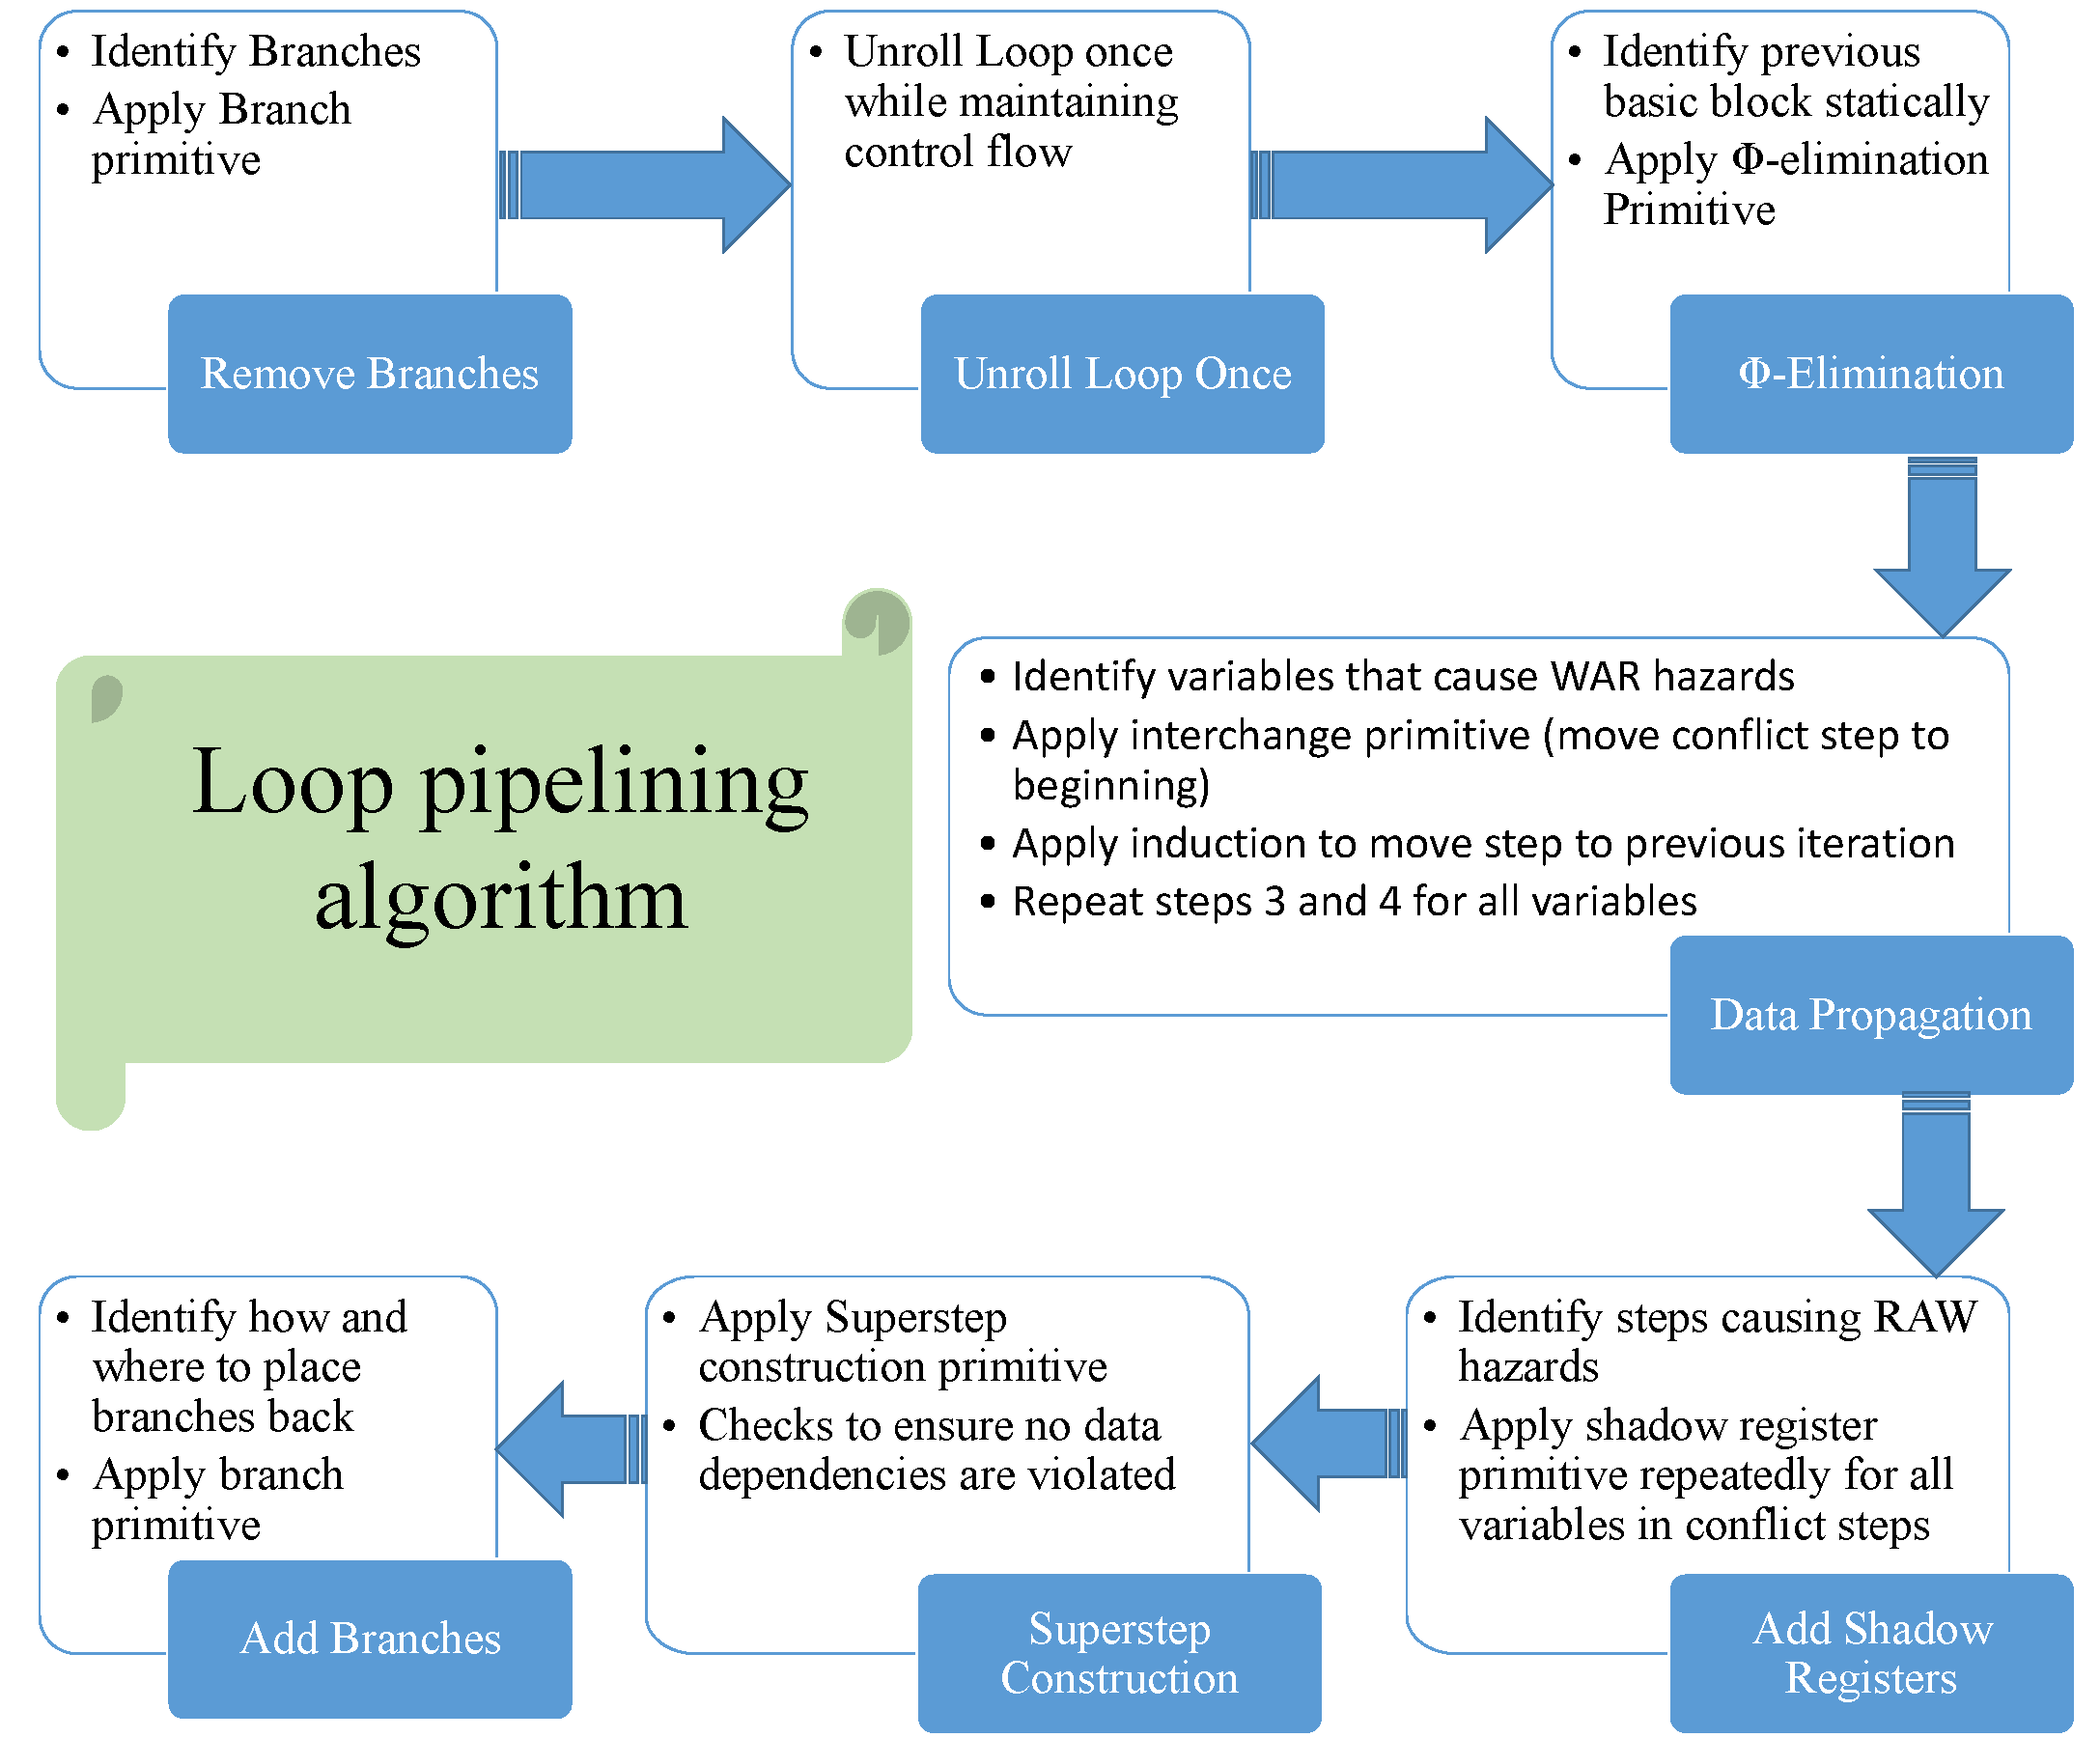
\includegraphics[height=1.8in]{fig-proposal/algorithm-using-primitives}
\\
(a) &  (b) 
\end{tabular}
\end{center}
\caption{(a) Branch Primitive (b) Algorithm Using Primitives}
\label{fig:branch-primitive}
\end{figure}

{\textbf {Branch primitive}} -- Branch instructions are required for control flow. However, reasoning about 
execution of branch instructions in a loop everytime we apply a primitive can make proof very complex.
We note that if we specifically assume that the exit condition becomes true after completing $k$ iterations, then we can remove the conditional branch.
To understand the branch primitive (c.f. Figure~\ref{fig:branch-primitive}), 
let's assume there is a conditional branch in the sequential loop structure $S$, which points to either
the next microstep in sequence or exits the loop by branching to the scheduling step
$Exit$. Let $S_{preExit}$ be the collection of microsteps before this branch in $S$ and
let $S_{loop}$ be the corresponding CCDFG loop without the conditional branch.
The conditional branch primitive allows us to replace $S$ with $S_{loop}$ followed by
$S_{preExit}$. Similarly,
the primitive also allows us to introduce an exit conditional branch by replacing
$S_{loop}$ followed by $S_{preExit}$ with $S$.
Note that since $k$ can take any value $k \ge 0$, we are not compromising on the correctness statement.  
It can be proved that executing $S$ such that it exits in the $(k+1)$ st
iteration is same as executing $S_{loop}$ $k$ times followed by $S_{preExit}$.

{\textbf {Interchange primitive}} -- Let $m$ and $n$ be two adjacent scheduling steps (or collection of microsteps) in a CCDFG where both $m$ and $n$ do not have read hazards and any microsteps containing branch statements. Then, the interchange primitive allows us to interchange their order without affecting execution. 

{\textbf {Superstep construction primitive}} -- This entails combining the scheduling steps of the successive
iterations, forming scheduling ``supersteps'' that act as scheduling steps for the pipelined implementation. Supersteps must
account for read-after-write hazards, i.e, if a variable is written in a scheduling step $X$ and read subsequently in
$Z$ then $Z$ cannot be in a superstep that precedes $X$ in the control/data flow.  Note that we implement data
forwarding (forward value of data within a single clock cycle); thus $X$ and $Z$ can be in a single superstep.

\subsection{Our Loop Pipelining Algorithm}

Given a sequential loop $S$ in CCDFG $C$ and pipeline interval $I$, we can create a pipelined loop $P$ using Algorithm~\ref{algo:loop}. Note that every step of the algorithm is build from ground up using our framework of provable primitives such that the algorithm can be certified by theorem proving (c.f. Figure~\ref{fig:branch-primitive} (b)). 

\begin{algorithm}[H]
\caption{Pipelining Algorithm}
\label{algo:loop}
\begin{algorithmic}[1]
\Procedure{PipelineLoop}{S, I}
\State $S_1 \leftarrow RemoveBranches(S)$
\State $S_2 \leftarrow UnrollLoopOnce(S_1)$
\State $S_3 \leftarrow \phi-Elimination (S_2) $.
\State $S_4 \leftarrow DataPropagation (S_3, I) $.
\State $S_5 \leftarrow GenerateShadowRegisters (S_4, I) $.
\State $ S_6 \leftarrow SuperstepConstruction (S_5, I) $.
\State $P \leftarrow AddBranches (S_6) $
\State \textbf{return} $(P)$.
\EndProcedure
\end{algorithmic}
\end{algorithm}

Now, we describe the steps to convert a sequential loop CCDFG $S$ (c.f. Figure~\ref{fig:branch-primitive}) to a pipelined loop CCDFG:

{\bf Remove Branches}: We apply the branch primitive on $S$ to remove branches by explicitly defining the control flow. 

{\bf Unroll Loop Once}: The first iteration behaves differently than the rest due to $\phi$-construct. So, we unroll the loop $S_{loop}$ once and call it $S_{pre}$. 

{\bf $\phi$-elimination}: We apply the $\phi$-elimination primitive on $S_{pre}$, $S_{loop}$ and $S_{preExit}$ to return a CCDFG in which all the $\phi$-statements have been replaced with their corresponding assignment statements. 

\begin{algorithm}
\caption{Data propagation} 
\label{algo:data-propagation}
\begin{algorithmic}[1]
\Procedure{DataPropogration}{$L$}
\State $msteps \leftarrow GetLoopCarriedDependencies(L)$
\For {\textbf{each} mstep \textbf{in} msteps}
\If {$CheckConflict (L, mstep, N, I) \neq 0$}
\State $L \leftarrow RelocateMStep (L, mstep)$
\EndIf
\EndFor
\State \textbf{return} $(L)$
\EndProcedure
\end{algorithmic}
\end{algorithm}

{\bf Data propagation:} Algorithm~\ref{algo:data-propagation} describes how to compute candidates for data
propagation across pipeline iterations. It is a critical step as we want to make sure that when we pipeline a loop, we do not read a variable which has not
yet been written. A critical observation is that data propagation is required only for loop carried dependencies.
$GetLoopCarriedDependencies$ identifies the microsteps where loop carried dependencies are being read. Then,
$CheckConflict$ checks whether there would be a conflict when we pipeline the loop. Conflict occurs when the value being read in a microstep is not yet written in the pipelined loop execution. If so, $RelocateMSteps$ relocates the microstep which is causing the data hazard to the previous iteraton. Note that this step requires multiple applications of interchange primitive and very complex induction. This step ensures that any variable which is being read has already been written. Note that in order to maintain the invariant, only those microsteps can be propagated which exist in $S_{preExit}$, which means only those steps which occur before the conditional branch in original CCDFG can be relocated. This ensures that our algorithm does not have the bug which the previously proposed algorithm had. In Figure~\ref{fig:algo1-3}(b) we found that the loop carried dependency $i'$ in $X$ would create a conflict when we would move $X$ before $Z$ while pipelining. So, we relocate the microstep $i := i'$ as shown in Figure~\ref{fig:algo2-2}(a). This step needs to be repeated for every variable found using $GetLoopCarriedDependencies$.

\begin{figure}[t!]
\begin{center}
\begin{tabular}{cc}
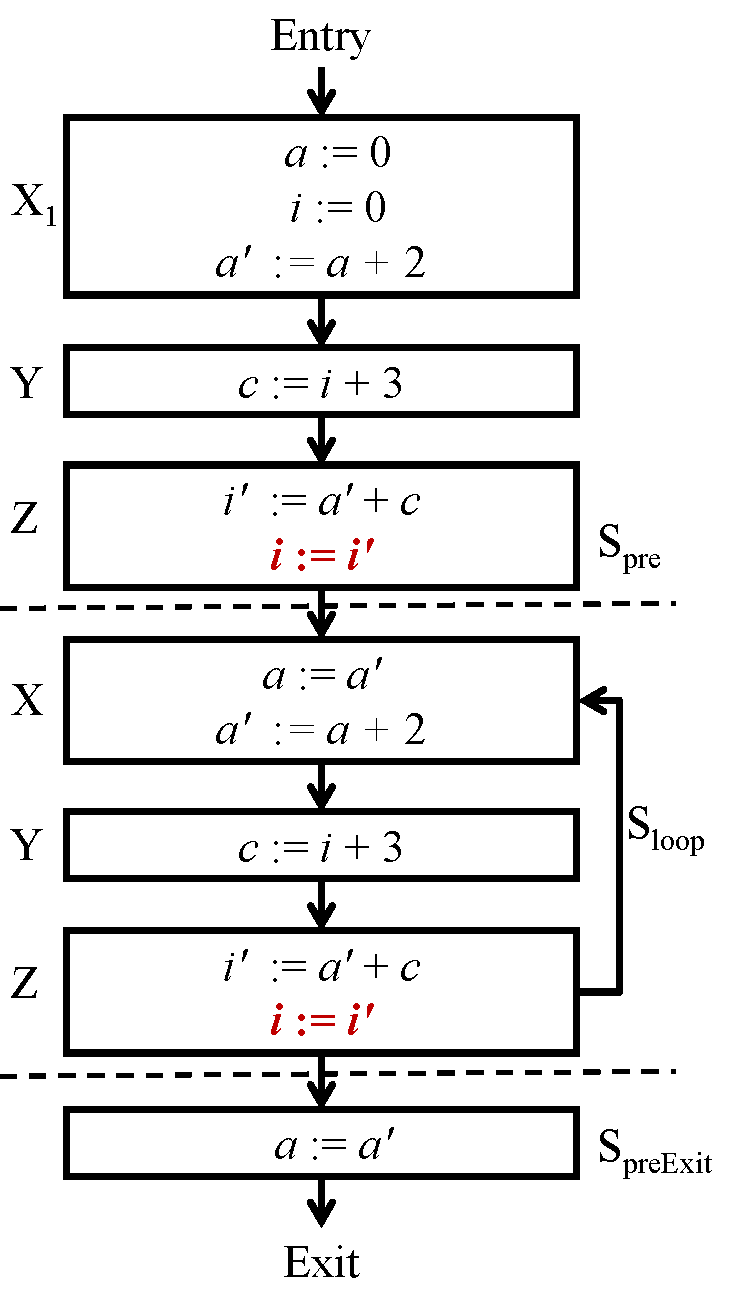
\includegraphics[height=2.5in]{fig-proposal/algorithm-after-data-propagation-2}
&
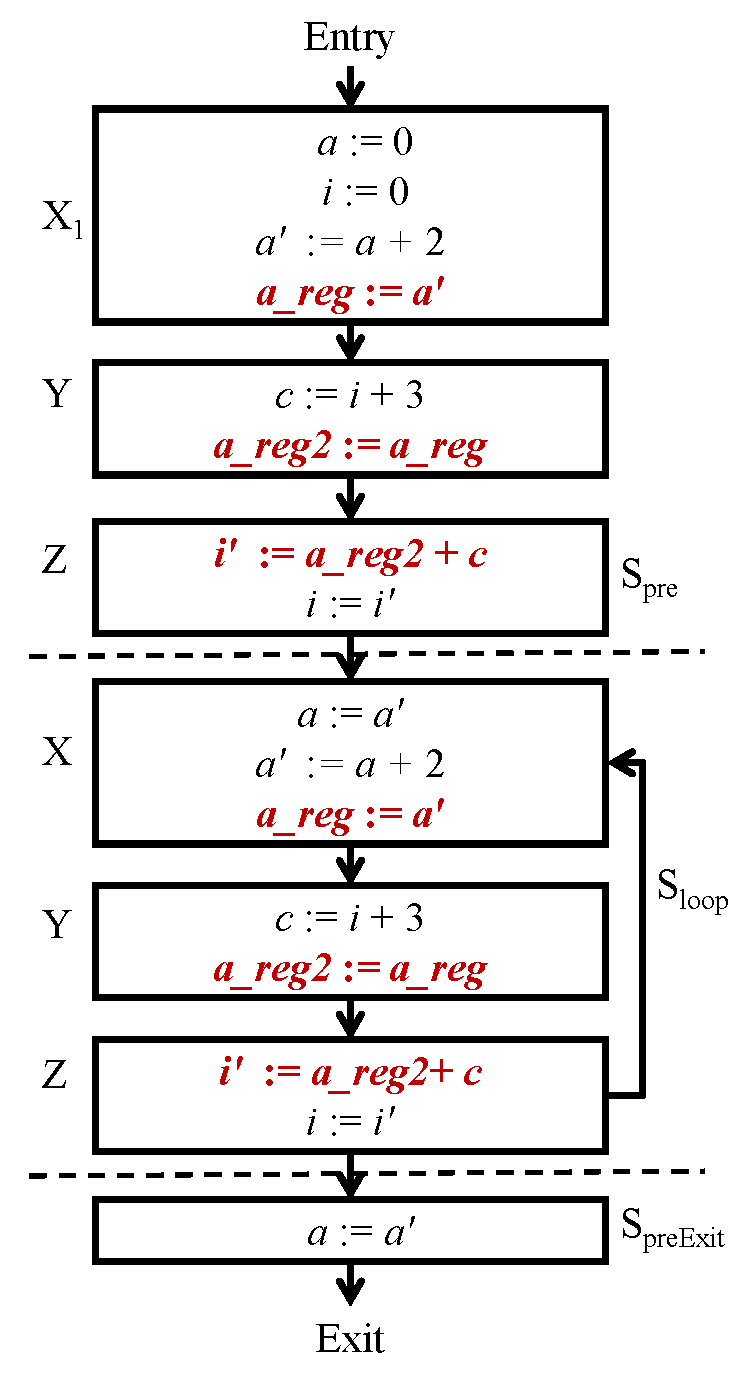
\includegraphics[height=2.5in]{fig-proposal/algorithm-after-shadow-register}
\\
(a) & (b)
\\
\end{tabular}
\end{center}
\caption{(a) After Data Propagation (b) After adding Shadow Register}
\label{fig:algo2-2}
\end{figure}

{\bf Generate shadow registers:} Algorithm~\ref{algo:generate-pipeline-registers} inserts shadow registers
to prevent variables from being overwritten before being read. We first compute all program variables that may be
overwritten before being read, which means these are the variables that require shadow registers. To find such variables,
 $GetAllVariables$ first gets a set of all variables. Then, for each variable, we compare the distance (the number of scheduling steps) between the write of
  the variable $w_v$ $(WriteVariable)$ and the last read of the variable $r_v$ $(LastReadVariable)$ in an iteration; if the
   distance is greater than $I$ (pipeline interval), the variable is assigned the new data value of the next iteration before the current iteration's value
    has been fully consumed; this warrants insertion of shadow registers in every scheduling step between the $r_v$ and $w_v$. The value is propagated every clock cycle following the CCDFG data flow. In Figure~\ref{fig:algo2-2}(b), we introduce a shadow register $a\_reg$ in $X$ and $a\_reg2$ in $Y$. This step is also repeated for all the variables found using $GetAllVariables$.

\begin{algorithm}[H]
\caption{Generate shadow registers} 
\label{algo:generate-pipeline-registers}
\begin{algorithmic}[1]
\Procedure{GenerateShadowRegisters}{$L$, $I$}
\State $V \leftarrow GetAllVariables(L)$.
\For {\textbf{each} v \textbf{in} V}
\State $w_v \leftarrow WriteVariable (v, L)$.
\State $r_v \leftarrow LastReadVariable (v, L)$.
\If {$RequireShadowRegister (r_v, w_v, I) \neq 0$}
\State $L \leftarrow AddShadowRegister (w_v, L)$.
\EndIf
\EndFor
\State \textbf{return} $(L)$.
\EndProcedure
\end{algorithmic}
\end{algorithm}



\begin{figure}[t!]
\begin{center}
\begin{tabular}{cc}
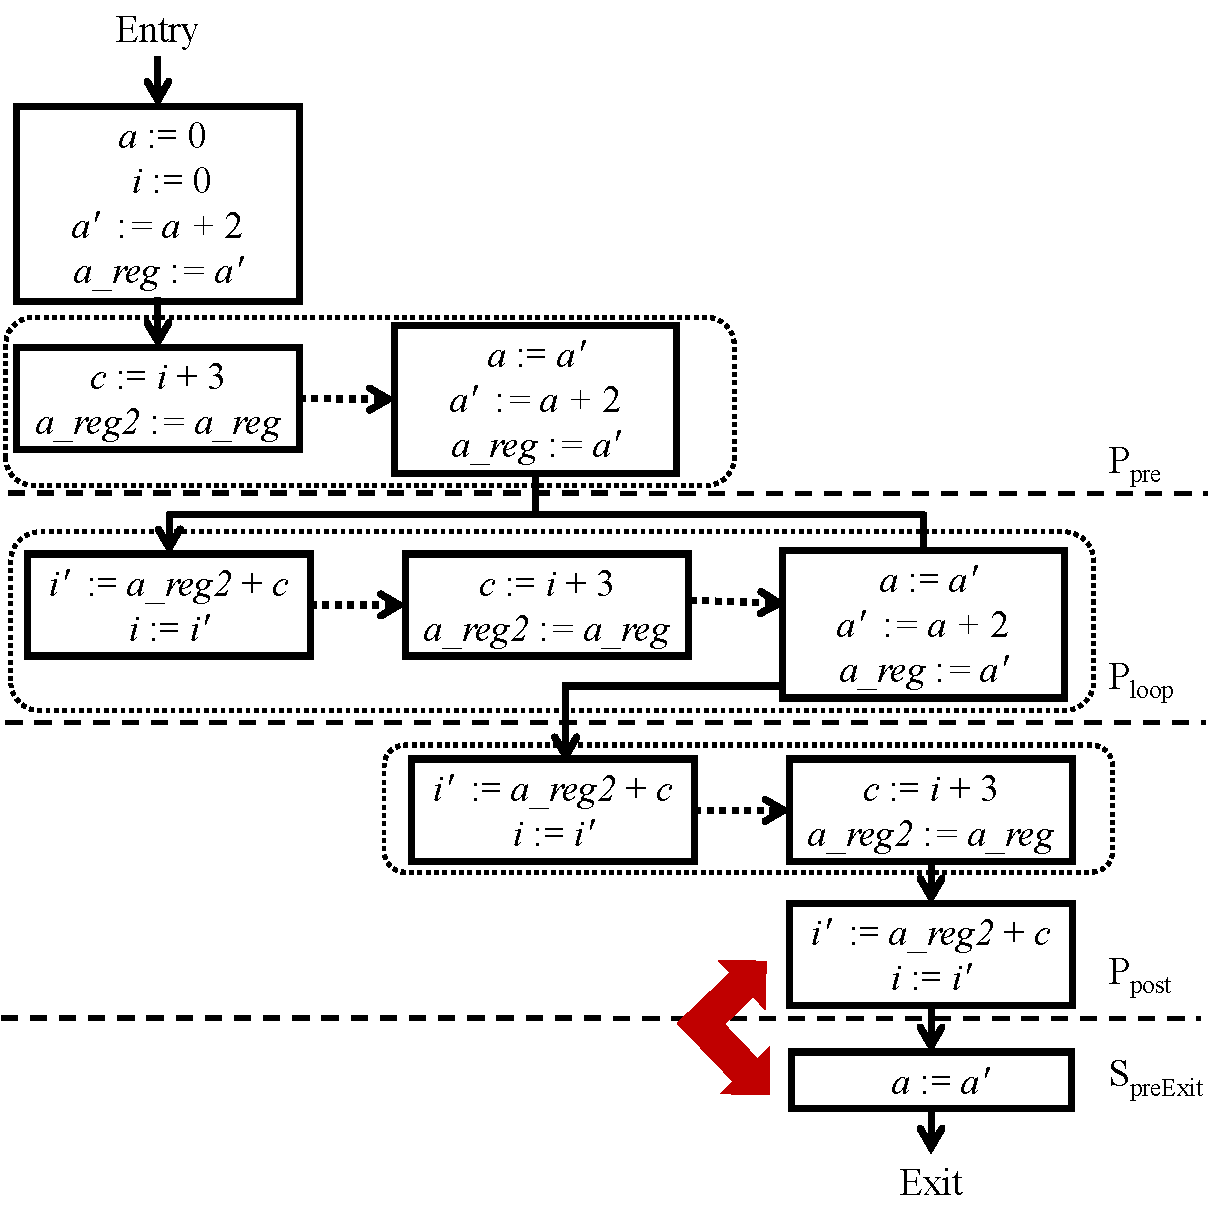
\includegraphics[height=2in]{fig-proposal/algorithm-after-superstep-construction}
&
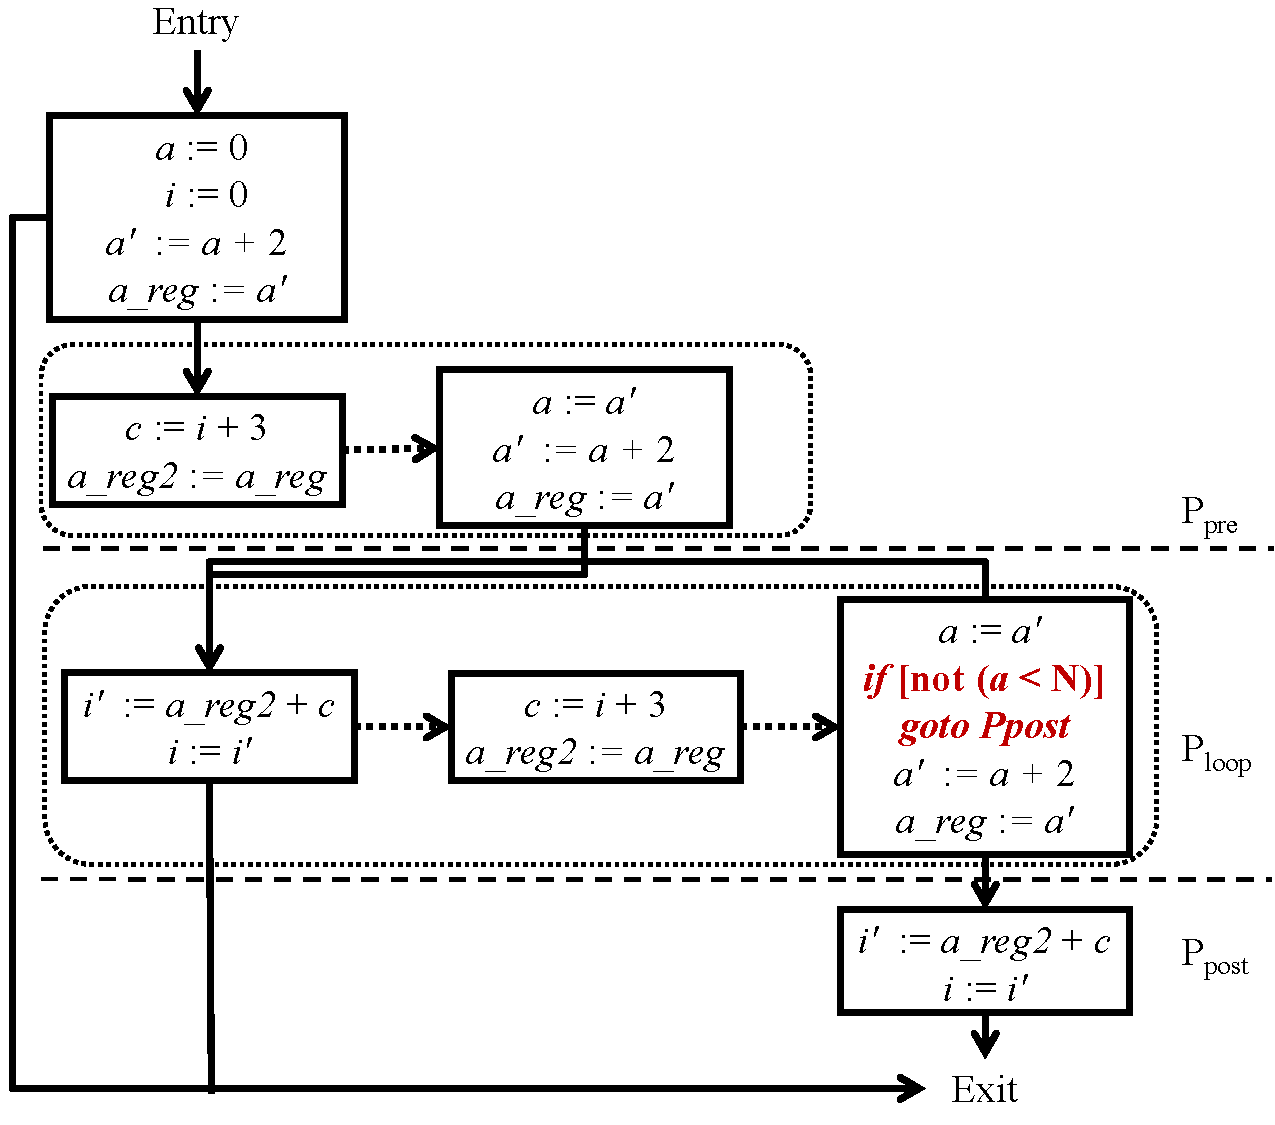
\includegraphics[height=2in]{fig-proposal/algorithm-after-adding-branches}
\\
(a) & (b)
\\
\end{tabular}
\end{center}
\caption{(a) After superstep construction (b) Final Pipelined CCDFG}
\label{fig:algo3-2}
\end{figure}

{\bf Superstep construction:} Now that we have removed the data hazards, we can successfully pipeline the loop using  the pipeline interval $I$. We combine the scheduling steps of the successive iterations, forming scheduling ``supersteps'' that act as scheduling steps for the pipelined
implementation. A scheduling step is allowed to move up another scheduling step only if there are no intermediate read and write conflicts. Note that we implement data forwarding; thus $s$ and $s'$ can be in a single scheduling superstep.
Superstep construction on $S_{pre}$ and $S_{loop}$ creates a CCDFG with three parts: prologue $P_{pre}$, $P_{loop}$ which is the full pipeline stage and epilogue $P_{post}$ as shown in Figure~\ref{fig:algo3-2}. 

{\bf Add Branches:}  To add the branches back, we use the a combination of interchange primitive and reverse of Branch primitive. Note in Figure~\ref{fig:algo3-2}, if there are no read write hazards in between the last scheduling step $Z$ of $P_{post}$ and $S_{preExit}$, we can interchange them using interchange primtive. Now recall from the branch primitive that if there is a loop structure $S_{loop}$ with a conditional branch, then executing $S_{loop}$ such that it exits in the (k+1)st iteration is same as executing $S_{loop}$ without the conditional branch followed by only those steps from $S_{loop}$ which occur before the branch $S_{preExit}$. Now, we apply the reverse of branch primitive here. $P_{loop}$ in Figure~\ref{fig:algo3-2} is a loop structure without a conditional branch, followed by a collection of microsteps $P_{preExit}$ (here, a collection of $Z$, $Y$ and $S_{preExit}$). Then, we can add an exit conditional branch in $P_{loop}$ after the microsteps $P_{preExit}$. This branch points to the next scheduling step after the loop $P_{post}$ if the exit condition is true. We can add the conditional and the unconditional branch as shown in  Figure~\ref{fig:algo3-2}(b).  

We now have the final pipelined loop structure. We describe a proof sketch for the primitives and the algorithm in the next section.

\section{Proof Sketch}
\label{sec:proof}

Certification of our loop pipelining algorithm naturally requires a certification of each of our primitives. In addition, we need to ensure that every time a primitive needs to be applied, the conditions under which the primitive can be applied are maintained. We discuss both aspects below.

\subsection{Correctness of Primitives}
We prove that applying a particular primitive is correct, 
{\em i.e.}, maintains a certain invariant. This proof does not 
consider how it is applied in the context of a pipeline
synthesis algorithm. In {\em $\phi$-elimination primitive}, we prove that the algorithm 
correctly resolves the $\phi$ to create multiple assignment statements. 
We induct along the length of each sub-microstep of $\phi$-construct and
relate it to one corresponding assignment statement. 
In {\em Shadow register primitive}, we prove that adding a shadow register microstep, $a\_reg = a'$ 
does not change the value of any variable in the state except the shadow variable. In essence, we prove
that if a variable is not written in a microstep, then its value in the state before and after executing
that microstep is same. Also, we prove that after executing the shadow register microstep,
value of $a\_reg$ in the state is equal to value of $a'$. Furthermore, since now
the value of $a\_reg$ is equal to value of $a'$, we prove that executing a statement which reads $a'$ has the same
effect on the state as executing a statement which reads $a\_reg$ till the next write of $a'$. This needs to be done for all types of
  statements {\em e.g.,} assignment statements (with different types of 
  operations like load, add, mul, getelementptr {\em e.t.c.}), 
  store statement, branch statement etc. We determine the variables read and 
  written in a statement by analyzing the statements. 
  Note that $a\_reg$ is a new variable which
  is neither written nor read in the given statements. In {\em Interchange primitive}, we prove 
  that we can interchange any two adjacent microsteps
 (excluding branch microsteps) which do not have read-write conflict by reasoning about execution
  semantics of all types of microsteps present in the
  language. In {\em Branch primitive}, we prove that executing $S$ such that it exits 
in the $(k+1)$ st iteration is same as executing $S_{loop}$ $k$ times followed by $S_{preExit}$. 
We need to define a notion of a well-formed-flow to ensure that we can show that the 
branch does not exit in the first $k$ iterations. We also need to track the backedge along the 
unconditional branch and ensure that it points back to the beginning of loop $S$.
 {\em Superstep construction primitive} is for overlapping iterations while 
maintaining data and control dependencies. It is built on interchange primitive but while interchange primitive
handles only two adjacent microsteps, superstep construction moves around scheduling steps with multiple microsteps. 
The interchange primitive is extended by non-trivial induction along the length of the scheduling steps to achieve the desired result. 
Superstep construction primitive is proved using the interchange primitive and a key invariant 
on correspondence between back-edges of sequential and pipelined loops~\cite{disha-itp14}. 

\subsection{Correctness of Our Algorithm}

%Following is an English paraphrase of the final theorem.
  
%\begin{quote}  
%If the pipeline generation succeeds without error,
%executing the pipelined CCDFG (a combination of $pre$, $loop$ and $post$) for $no\_pp\_steps$
%generates the same state of the relevant variables as executing the sequential CCDFG $c$ for $no\_seq\_steps$.
%\end{quote}
%\small
%\begin{equation}
%\begin{split}
%no\_seq\_steps &= len S_{1} + (len S * (\ceil{\frac{m}{interval}} - 1)) + len S_{preExit} \\
%no\_pp\_steps &= len P_{pre} + (len P_{loop} * k) + len P_{post}
%\end{split}
%\end{equation}

The algorithm is essentially built from ground-up using primitives
as shown in Section~\ref{sec:pipelining-algorithm}. However, 
apart from proving correctness of each primitive and our key 
invariant, we also need to ensure that the primitive is applied by 
our algorithm properly, {\em i.e.}, the environment
assumptions on which the {\em correctness of primitive}
depends are maintained appropriately by the algorithm at
the point where the primitive is applied. We can take each stage one by one to understand the complexity involved in 
verifying the algorithm as a whole, over and above the verification of 
individual primitives. In the $Remove Branches$ stage, which is the first stage of pipelining algorithm, 
we have to create a correspondence between randomly executing a CCDFG with branches using basic-block, 
sub-basic-block and location with executing a CCDFG in sequence without a conditional and unconditional branch. 
After this step and for all the subsequent steps, we need to show that there are no relevant branches in CCDFG. 
In the $\phi$-to-assign stage, we replace one microstep of $C$ with more than one microsteps in $C'$. 
An inductive statement showing the correctness of $\phi$-elimination must account for the fact
that the number of microsteps of $C$ is different from that
of $C'$.  Thus an execution of $C$ for $n$ microsteps must
correspond to an execution of $C'$ for a different number
$m$ of microsteps, where the number $m$ is a function of $n$
and the structures of $C$ and $C'$; the statement of the
correctness of $\phi$-elimination must characterize the
value of $m$ precisely, perhaps defining functions that
statically and symbolically execute $C$ and $C'$, in order
to be provable by induction.  Furthermore the functions so
introduced for static symbolic execution must themselves be
proven correct. $Data propogation$ involves identifying 
the appropriate statements that cause conflict and applying 
interchange primitive multiple times 
to move the microstep to the beginning of the loop. 
We need to make sure that the conditions under which
interchange primitive can be further applied are maintained after each application. 
$Shadow register step$ also adds many more new statements to assign temporary values to 
new shadow variables. The addition of new microsteps means that in addition to 
inductively reasoning about application of a primitive in entire CCDFG, we also have to 
ensure that basic structure of the CCDFG is maintained. Moreover, we need to reason about read and write of 
variables across a number of microsteps. The proof is analogous to the proof of shadow-register primitive. 
However, the primitive is applied multiple times based on the variabes which are causing conflict. 
This gets tricky as after application of one primitive, there are new variables introduced and 
we can only claim that the relevant variables have same value.This step requies proof of invariant and multiple applications of interchange primitive as explained earlier. The proof required is the reverse of branch-primitive. However, a key requirement is that branch-primitive can be applied only when we have a {\tt well-formed-ccdfg}, so we need to ensure that the structure of the $loop$ before adding 
branches is such that the final $loop$ in the pipelined CCDFG is indeed a {\tt well-formed-ccdfg}.  


\section{Viability of our Approach}
\label{sec:SEC}

We have successfully tested the pipeline reference model generated by our certified algorithm with that generated by the previous algorithm~\cite{kechengthesis} across several industrial strength designs in different domains(c.f Figure~\ref{fig:testing}). The designs are non-trivial to pipeline with varied pipeline intervals and depths.

\begin{figure}
\begin{center}
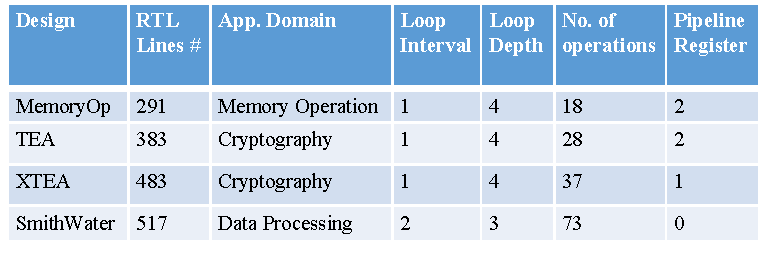
\includegraphics[height=1.5in]{fig-proposal/testing}
\end{center}
\caption{Behaviorally synthesized pipelined designs tested using our algorithm}
\label{fig:testing}
\end{figure}









\section{Related Work and Novelty of Our Approach}
\label{sec:related-work}

Besides behaviorally synthesized pipelines, there are mainly two other kinds of pipelines, hardware pipelines and software pipelines. 
There has been a significant amount of work in verification of hardware pipelines~\cite{pvs,Cyrluk94, bd:pipeline, sh:pipeline}. 
There are significant differences in goals
and techniques between these efforts and ours.
Microprocessor pipelines include optimized (hand-crafted)
control and forwarding logics, but have a static set of
operations based on the instruction set. Behaviorally synthesized 
loop pipelines tend to be deep with a high complexity at each stage, but
control and forwarding logics are more standardized since
they are automatically synthesized. 
Furthermore, microprocessor pipeline verification
is focused on one (hand-crafted) pipeline implementation,
while our work focuses on verifying an {\em algorithm
that generates pipelines}. Our invariant is very different from a typical invariant
used in the verification of pipelined machines~\cite{sh:pipeline} . We make explicit the
correspondence with the sequential execution. The key
requirement from a pipeline invariant, \viz, hazard freedom,
is left implicit and arises indirectly as a proof obligation
for invariance of this predicate. 
 
Behaviorally synthesized loop pipelines are similar in reasoning to software loop pipelines except that since
behavioral synthesis is automatic, it is much more streamlined than software pipelines. 
Our understanding of hazards and reasoning behind pipelining algorithm 
is very closely related to verification of software pipelines.  In particular, Tristan
and Leroy~\cite{tl:software-popl10} present a verified
translation validator for software loop pipelines.  The loop
pipelines in behavioral synthesis considered in this paper
are close in structure to software loop pipelines, although
our formalization (\eg, CCDFG) has different semantics from
the Control Flow Graphs they use, reflecting the difference
between eventual targets of compilation (\viz, hardware
vs. software).  However, the fundamental difference is in
the approach taken to actually certify the pipelines.
Tristan and Leroy's approach decomposes the certification
problem into two parts, a ``dynamic'' part that is certified
on a case-by-case basis  and a ``static'' part that is
certified in the Coq theorem prover~\cite{coq} once and for all.  The
theorem proven by Coq is informally paraphrased as follows:

\begin{quote}
Suppose the pipelining algorithm generates a pipeline
${\cal{P}}$ from a sequential design ${\cal{S}}$.  Suppose
symbolic simulation of ${\cal{S}}$ and ${\cal{P}}$ verifies
certain ``dynamic'' verification conditions (VCs).  Then
${\cal{S}}$ and ${\cal{P}}$ are indeed semantically
equivalent.
\end{quote}

\noindent
Thus for any pipeline instance ${\cal{P}}$ generated by
their algorithm, symbolic simulation is executed between
${\cal{P}}$ and ${\cal{S}}$ to certify that ${\cal{P}}$ is
indeed a correct pipelined implementation of ${\cal{S}}$.
The dynamic VCs checked by symbolic simulation essentially
certify that the pipeline generation did not overlook any
hazards.

This is where our work differs from theirs.  Our work is
expected to provide a single theorem certifying the
correctness of the reference pipelined implementation,
without requiring further runtime hazard check.
Furthermore, their correspondence theorem relates the
pipelined implementation with a sequential design with a
(bounded) unrolled loop, while our approach certifies the
correspondence between the actual Control Flow Graph (CFG)
and the pipelined implementation.  Indeed, Tristan and Leroy
remark that the mechanization of the correspondence between
the CFG and unrolled loop is ``infuriatingly difficult''.
We speculate this is so because they focus on verifying the
correspondence between the unrolled loop and the pipeline.
In our experience, attempting the formal correspondence between the unrolled
sequential loop and pipelined design is indeed difficult since
there is no formal way to connect to back edge of the loop
with any of the edges in the pipeline.  We believe that
reconciling this problem and developing a fully certified
pipeline generation algorithm would require backtracking
from the correspondence with an unrolled loop (and hence
translation validation) to a more complex invariant like
ours.  Of course we must note that we can ``afford'' to
develop a fully certified algorithm in our approach since
the pipelines are simpler
(cf. Chapter~\ref{sec:formalization}); achieving this for
arbitrary software pipeline may require further more subtle
invariants.

\begin{comment}
%Thorem provers are widely used for hardware verification. 
%HOL theorem prover~\cite{hol} has been used in 
%several well-documented projects~\cite{cohn,graham}.
ACL2 is also used a lot in hardware 
verification~\cite{Russinoff,car2,car,Hardin,ray-abstracting,ray-connecting,ray-certification}. 
Our project is however somewhat different from the
traditional applications of theorem provers. 
First, since an over-arching goal is to exploit automatic
decision procedures, we use theorem proving primarily to
complement automated tools. Second, we eschew theorem
proving on inherently complex or low-level implementations.
Third, interactive theorem proving is acceptable for
one-time use, in certification of a transformation, 
but not as part of a methodology that
requires ongoing use in certification of each design. The
constraints are imposed by the the environment in which we
envision our framework being deployed: it may not be
possible to have a dedicated team of experts doing theorem
proving as full-time jobs. Finally, the loop pipelining transformation
we verify are proprietary to the synthesis tools. Therefore, our approach is
targeting verification of transformations
which are closed-source (and exceedingly complex), thus
making traditional program verification techniques unusable.
Our approach shows a novel way in which theorem
proving can be applied even under those constraints, in
concert with automated SEC.
\end{comment}

In addition to technical contributions, we see our work as
providing an important methodological contribution enabling
use of theorem proving in situations where one needs to
certify the result of an implementation on which theorem
proving cannot be directly applied either because it is
closed-source or because it is highly complex: (1)~create a
reference implementation, perhaps using as much information
as available from the actual implementation, in our case
information about pipeline intervals, (2)~certify this
simpler reference implementation with theorem proving, and
(3)~develop an SEC framework to compare the result of the
reference implementation with that of the actual
implementation.  In addition to making theorem proving
applicable on industrial flows without requiring us to
certify industial implementations with their full
complexity, this approach permits adjusting the algorithm
(within limits) to suit mechanical reasoning while still
affording comparison with actual synthesized artifacts.  We
have made liberal use of this ``luxury'', \eg, we have
been continually redefining our superstep construction function
to facilitate proof of key structural lemmas of the
invariant before settling on the final version.  We believe similar approach is applicable in
other contexts and may provide effective use of theorem
proving within industrial verification flows.

\section{Conclusion and Future Work}
\label{sec:research-plan}

We have developed a framework of succinct certified primitives essential to build pipelining algorithms. We utilize our framework of certified primitives as backbone to build our certified loop pipelining algorithm. Since, we have a certified loop pipelining algorithm, we can confidently say that there are no data hazards and executing a sequential loop is same as executing a pipelined loop created using our algorithm. We have tested the pipeline reference model created using our algorithm on a variety of industrial strength designs across different application domains. %This shows that our algorithm is practical and can be used for industrial strength designs with tens of thousands of RTL.  Our current ACL2 script has $296$ definitions and $1012$ lemmas, including many lemmas about structural properties of CCDFGs (but not counting those from the false starts). 

\begin{table}
  \centering
  \label{fig:proof}
  \begin{tabular}{| c | c |}
    \hline
    Definitions & 296 \\
    \hline
    Lemmas & 1012 \\
    \hline
  \end{tabular}
        \caption{ACL2 Effort}
\end{table}

%Our work shows that it is possible to develop and certify an industrial-strength loop pipelining algorithm if we can decompose it into succint certifiable primitives. We have already identified and certified these primitives. 
Our algorithm has components which can identify data hazards based on the given pipeline interval. Then we use our certified primitives to remove those data hazards and create a pipelined implementation. Function pipelining algorithms also have the same type of data hazards as we have mentioned in loop pipelining algorithms. However, while loop pipelines have a fixed pipeline interval which is known at compile time, function pipelines have a variable pipeline interval for every iteration. So, instead of identifying data hazards at once for every iteration, we would have to call those functions for each iteration. After we have identified the data hazards, we can use our certified primitives to remove those data hazards. We believe that if we can modify the algorithm to identify data hazards, then we can conveniently reuse our certified primitives to certify behaviorally synthesized function pipelines as well.     

\bibliographystyle{plain}
\bibliography{bib}
\end{document}
